\section{気体の状態変化(2)}

% 例題番号は原本と同じく第2章（熱力学）の通し番号を引き継ぐ（第16回が【例題8】〜【例題10】）
\setcounter{nombre}{10}

\subsection{熱力学第一法則と内部エネルギーの変化(2)}
% 加筆（2026-09-02）：原本 p78 の 17.1 にあたる節が TeX 版には無く，等温変化の
%   説明が丸ごと抜けていた（練習問題［26］・原本の例題11 が定温変化を問う）．
%   原本の導入文と，等温変化についての最低限の説明を補った．
前週に続き，温度一定の{\bf 等温変化}と，熱のやりとりをしない{\bf 断熱変化}について考える．

等温変化では温度が変化しないので内部エネルギーも変化せず，$\Delta U=nC_V\Delta T=0$である．
したがって熱力学第一法則$\Delta U=Q+(-w)$より$Q=w$，すなわち{\bf 加えた熱はすべて気体が外界にする仕事になる}．
また，等温変化の途中では圧力が体積とともに変化していくので，気体のする仕事は$w=P\Delta V$とは書けず，体積が$V[{\rm m^3}]$のときの圧力$P(V)$[Pa]を求めてから$w=\displaystyle\int P(V)dV$を計算しなければならない．

\begin{reidaiunit}
\begin{reidai}{等温変化}
\begin{zuright}{58mm}
\hspace{1zw}図のように一様な断面積を持つシリンダーに定積モル比熱が$C_V\U{J/mol\cdot K}$の理想気体を$n\U{mol}$封入した．ピストンは軽くて自由に動くことができ，棒が取り付けてある．最初，この気体の温度は$T_0\U{K}$，体積は$V_0\U{m^3}$であった．
\zusep
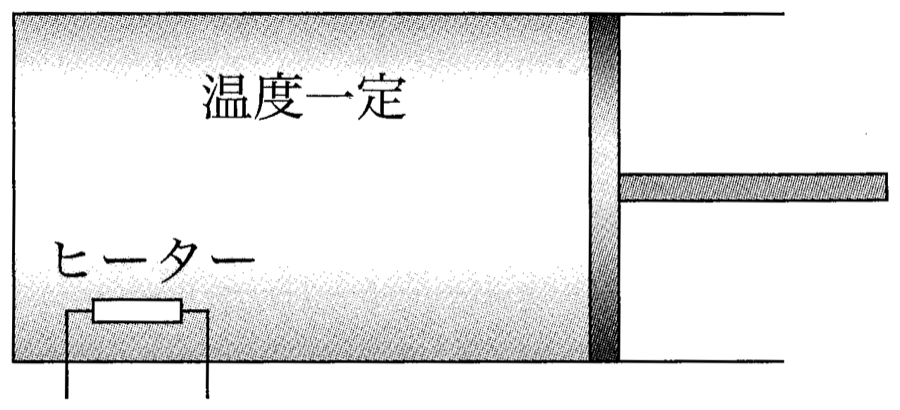
\includegraphics[keepaspectratio,width=58mm]{fig/ch17_ex11_cyl.png}
\end{zuright}
\hspace{1zw}シリンダー内にはヒーターが取り付けてあり，気体に対して熱を与えることができる．シリンダーおよびピストンは断熱材で出来ており，ヒーターによって与えた熱が大気に逃げることはないものとする．気体定数を$R\U{J/mol\cdot K}$として以下の問に答えよ．
\begin{komon}
\ko{1} 始めの状態における気体の圧力$P_0\U{Pa}$を求めよ．
\end{komon}
\hspace{1zw}ここで，気体が温度$T_0\U{K}$を保つようにピストンを操作しながら気体に熱をゆっくりと与え，体積を$V_1\U{m^3}$となるまで膨張させた．
\begin{komon}
\ko{2} 終状態における気体の圧力$P_1\U{Pa}$を求めよ．
\ko{3} 気体の体積が$V\U{m^3}$（$V_0<V<V_1$）のときの気体の圧力$P(V)\U{Pa}$を求めよ．
\ko{4} この状態変化を$P-V$図で表せ．
\ko{5} この変化において気体が外界に対してした仕事$w\U{J}$を求めよ．ただし，$\displaystyle\int\frac{1}{x}dx=\log|x|+C$（$C$は積分定数）である．
\ko{6} この変化における気体の内部エネルギーの増加量$\Delta U\U{J}$を求めよ．
\ko{7} ヒーターによって加えた熱量$Q\U{J}$を求めよ．
\end{komon}
\end{reidai}

\begin{sisinE}
温度が一定に保たれる状態変化を{\gtfamily 等温変化}という．等温変化では内部エネルギーが変化しないので，加えた熱はすべて気体が外界にする仕事になる．

(5) この状態変化では圧力$P$は一定ではないから，$w=P\Delta V$とは書けないことに注意せよ．体積が$V\U{m^3}$のときの圧力$P(V)$を求め，それを積分する．
\end{sisinE}

\Key{状態方程式 $PV=nRT$\quad 内部エネルギー変化 $\Delta U=nC_V\Delta T$\quad 気体のする仕事 $w=\displaystyle\int_{V_1}^{V_2}P\,dV$\quad 熱力学第一法則 $\Delta U=Q+(-w)$}

\begin{kaitou}
\begin{komon}
\ko{1} 始めの状態の状態方程式$P_0V_0=nRT_0$より，
       \Ana{P_0=\frac{nRT_0}{V_0}\U{Pa}\Ans}
\ko{2} 終状態でも温度は$T_0$のままであるから，状態方程式$P_1V_1=nRT_0$より，
       \Ana{P_1=\frac{nRT_0}{V_1}\U{Pa}\Ans}
\ko{3} 体積が$V$のときも温度は$T_0$であるから，状態方程式$P(V)\cdot V=nRT_0$より，
       \Ana{P(V)=\frac{nRT_0}{V}\U{Pa}\Ans}
\ko{4} (3)より$P-V$図は$PV=nRT_0$（一定）の双曲線の一部で，次図の通り．
       \begin{center}
       \ifbsAnaume
       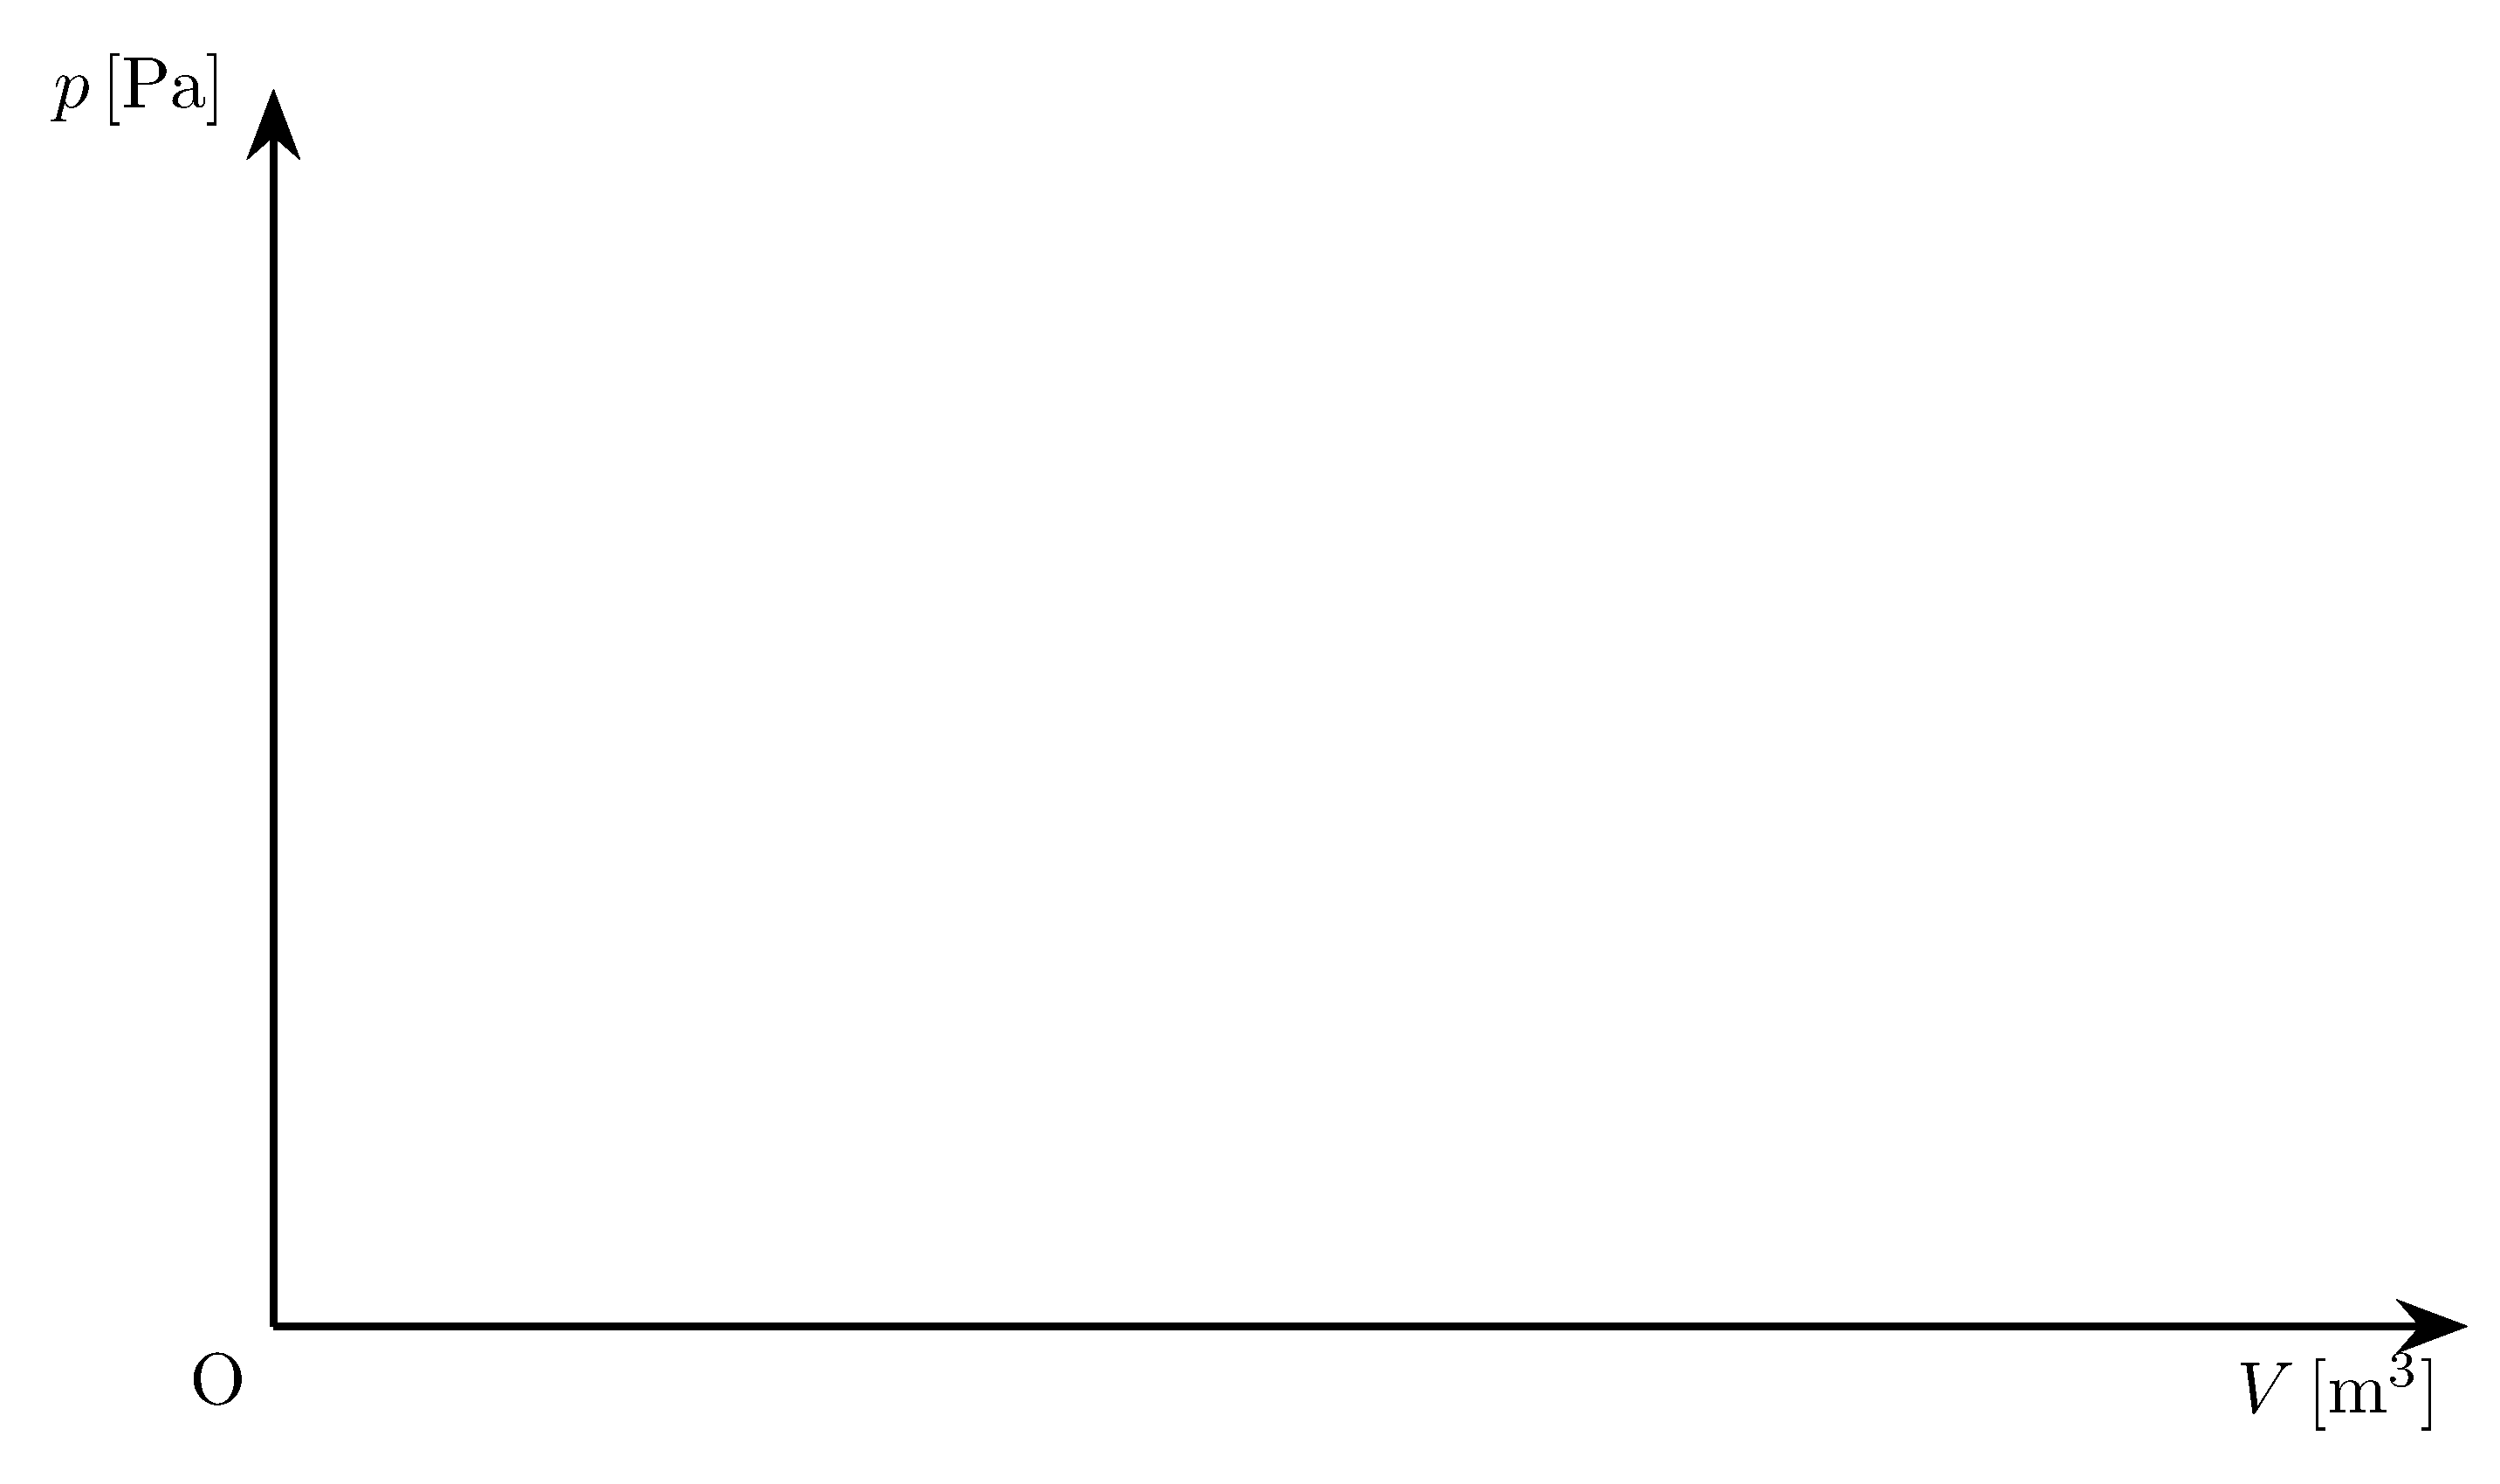
\includegraphics[keepaspectratio,width=96mm]{fig/ch17_ex11_pv_blank.png}
       \else
       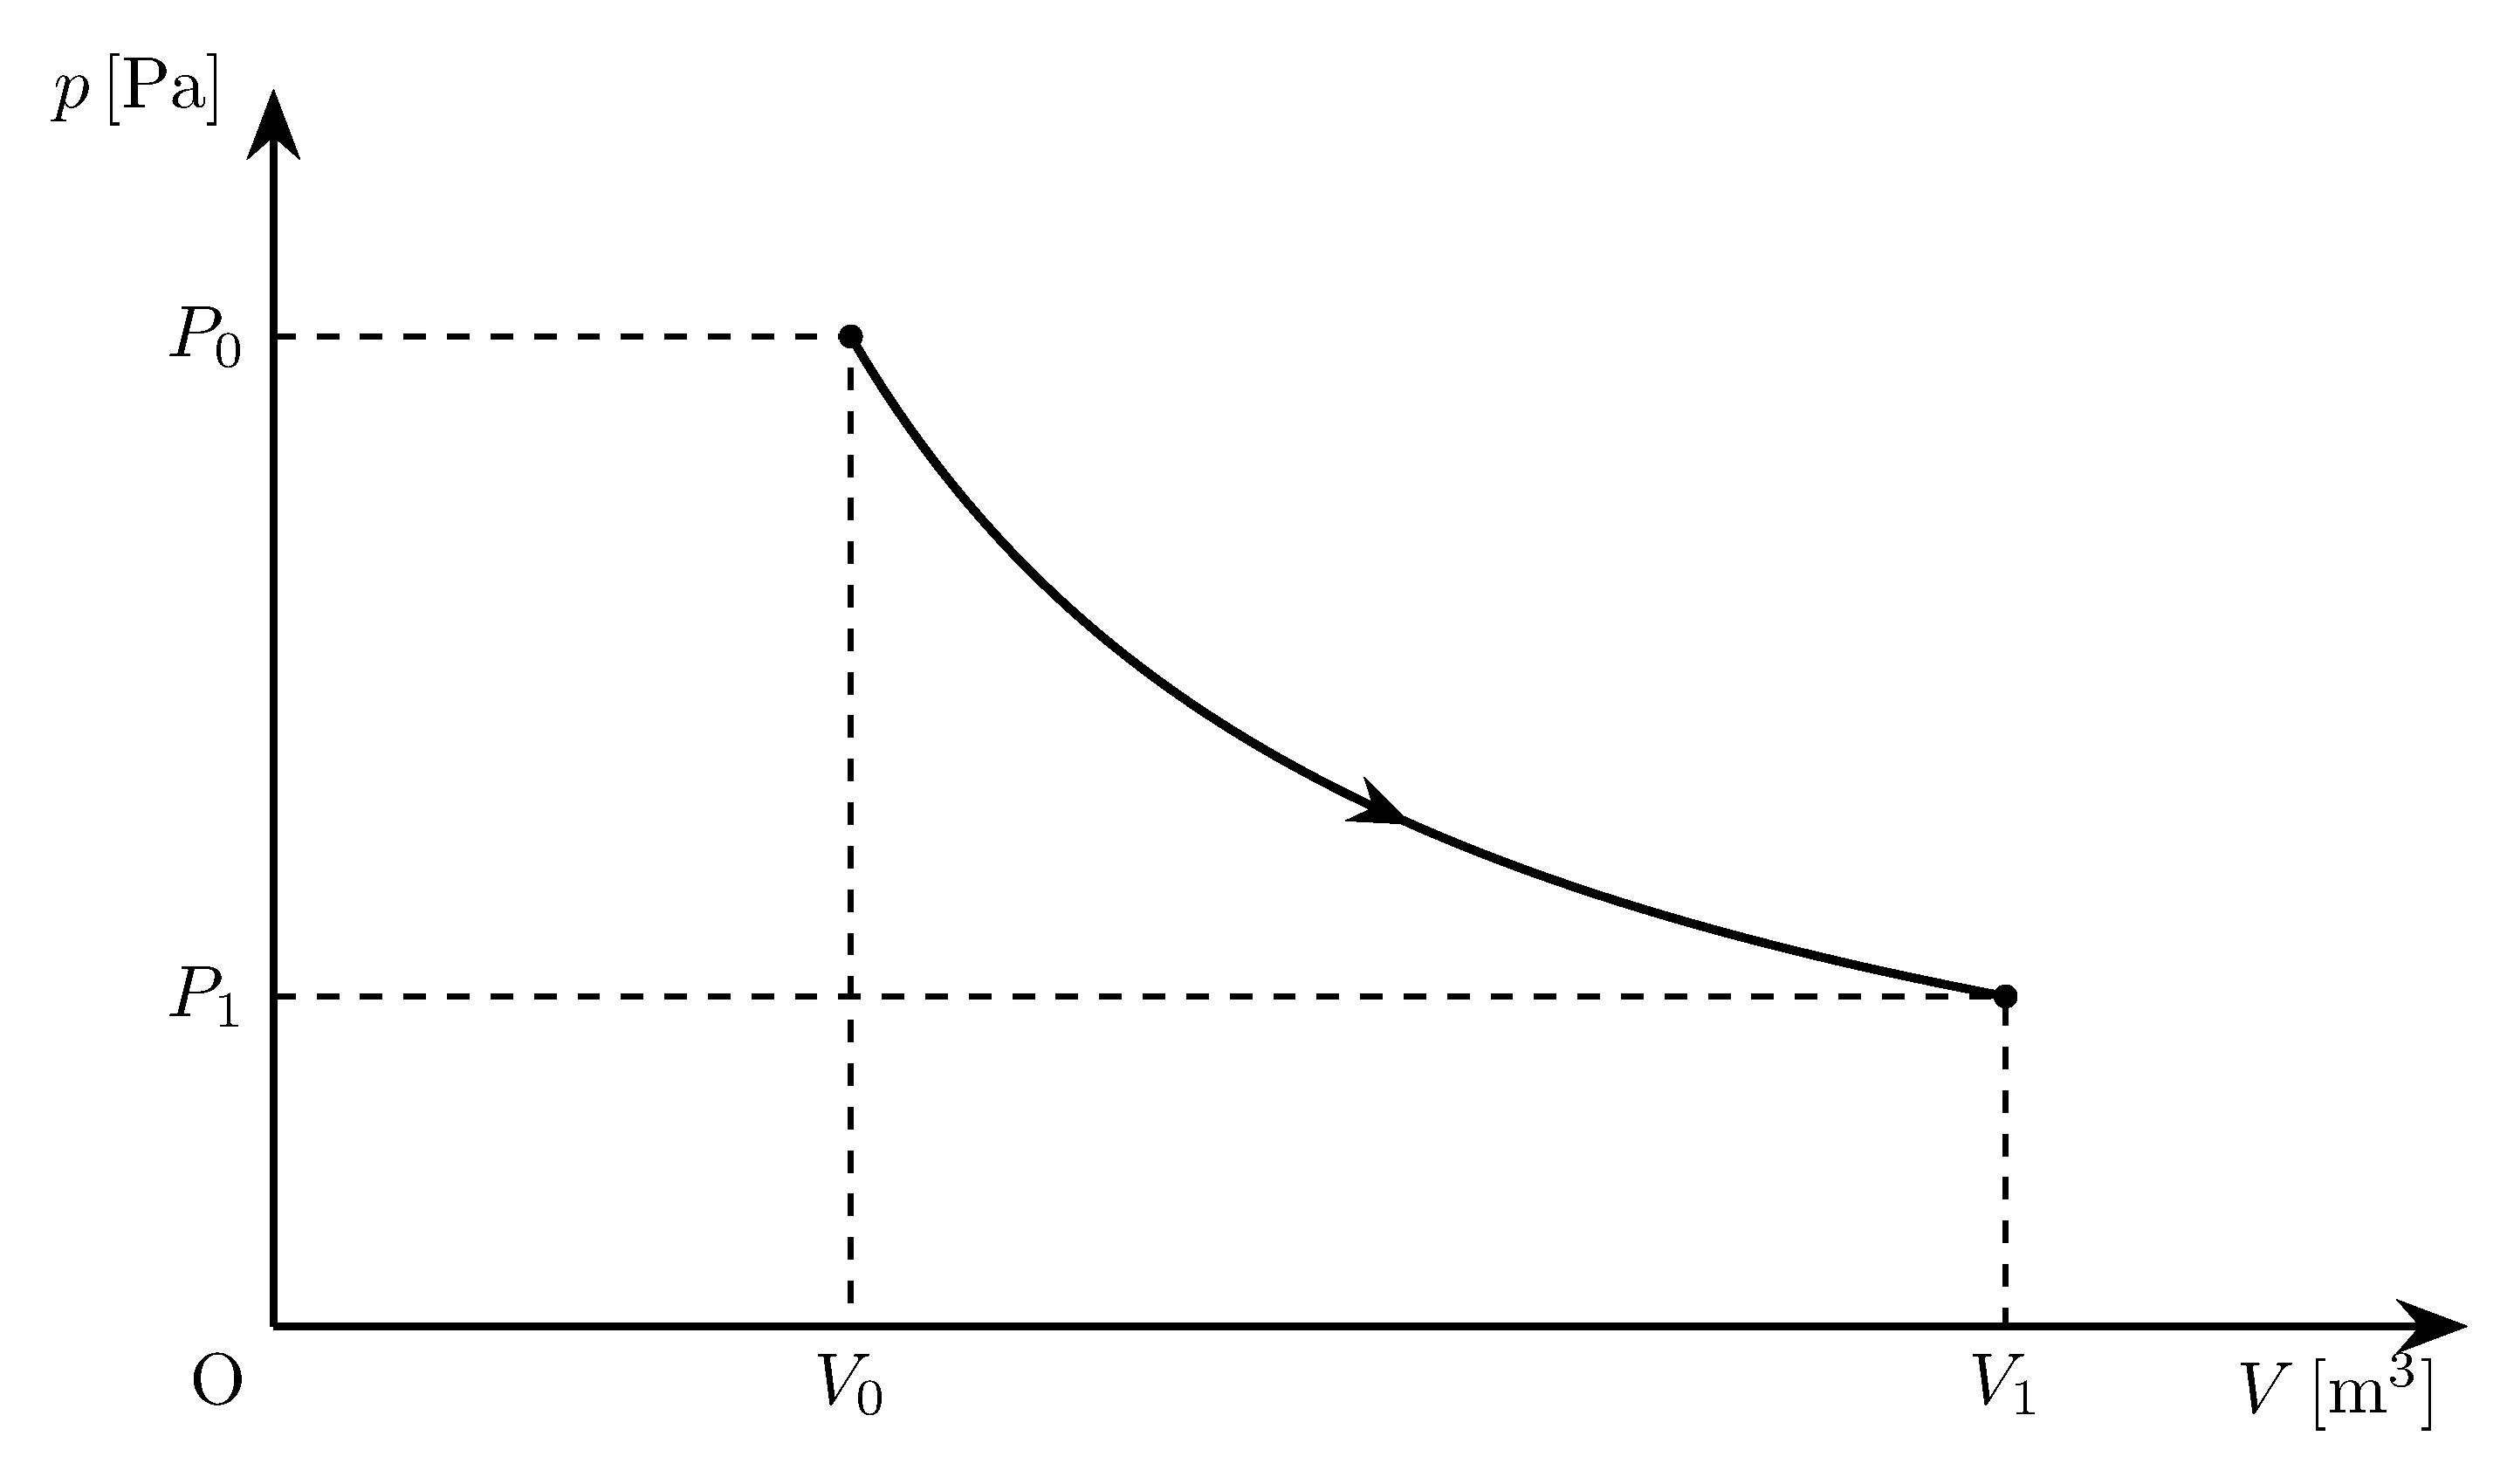
\includegraphics[keepaspectratio,width=96mm]{fig/ch17_ex11_pv.png}
       \fi
       \end{center}
       \hspace*{\fill}\Ans
\ko{5} $nRT_0$は定数であることに注意して，
       \Ana{w=\int_{V_0}^{V_1}P(V)dV=nRT_0\int_{V_0}^{V_1}\frac{1}{V}dV
             =nRT_0\log_e\frac{V_1}{V_0}\U{J}\Ans}
\ko{6} 温度が$T_0$のまま変化しないので$\Delta T=0$であり，
       \Ana{\Delta U=nC_V\Delta T=0\U{J}\Ans}
\ko{7} 熱力学第一法則$\Delta U=Q+(-w)$より，
       \Ana{Q=\Delta U+w=nRT_0\log_e\frac{V_1}{V_0}\U{J}\Ans}
       すなわち，加えた熱はすべて気体が外界にした仕事になっている．
\end{komon}
\end{kaitou}
\end{reidaiunit}


\subsection{断熱変化}
外部との熱の出入りを遮断して気体を状態変化させることを断熱変化という．
断熱変化では圧力，体積，温度の全てが変化する．

\begin{reidaiunit}
\begin{reidai}{断熱変化}
\hspace{1zw}始状態において圧力$P_0\U{Pa}$，体積$V_0\U{m^3}$の理想気体を，外部との熱のやり取りを断ったまま体積が$V_1\U{m^3}$（ただし$V_1>V_0$）になるまで変化させる．終状態における気体の圧力を$P_1\U{Pa}$，気体定数を$R\U{J/mol\cdot K}$，気体の定積モル比熱を$C_V\U{J/mol\cdot K}$として以下の問に答えよ．
\begin{komon}
\ko{1} 内部エネルギー変化$\Delta U\U{J}$，気体が外にした仕事$w\U{J}$，吸熱量$Q\U{J}$を求めよ．
\ko{2} 膨張過程なので$w>0$である事を利用して，この変化によって気体の温度は増加するか，減少するか，答えよ．
\end{komon}
\end{reidai}

\begin{sisinE}
熱の出入りを断った状態変化なので$Q=0$である．与えられているのは$P$と$V$だけで温度が与えられていないが，状態方程式$PV=nRT$を使えば$nRT$を$PV$に置き換えられるので，$\Delta U=nC_V\Delta T$は$P$, $V$だけで表せる．
\end{sisinE}

\begin{kaitou}
\begin{komon}
\ko{1} 断熱変化であるから，
       \[Q=0\U{J}\Ans\]
       気体のモル数を$n\U{mol}$，始状態・終状態の温度を$T_0\U{K}$, $T_1\U{K}$とすると，状態方程式より$P_0V_0=nRT_0$, $P_1V_1=nRT_1$であるから，
       \[\Delta U=nC_V(T_1-T_0)=\frac{C_V}{R}(P_1V_1-P_0V_0)\U{J}\Ans\]
       熱力学第一法則$\Delta U=Q+(-w)$に$Q=0$を代入して，
       \Ana{w=-\Delta U=\frac{C_V}{R}(P_0V_0-P_1V_1)\U{J}\Ans}
\ko{2} (1)より$\Delta U=-w$であり，$w>0$であるから$\Delta U<0$である．$\Delta U=nC_V\Delta T$で$nC_V>0$であるから$\Delta T<0$，すなわち気体の温度は\AnaU{\gtfamily 減少する}．\hspace*{\fill}\Ans
\end{komon}
\end{kaitou}
\end{reidaiunit}

% 加筆（2026-09-02）：原本 p79 の例題12 の直後の段落．例題12 を入れたので，
%   ポアソンの法則へつなぐ原本どおりの言い回しに戻した．
準静的な断熱変化では圧力，体積，温度の全てが変化するが，終状態は1通りしか取れないため，例題12の終状態の圧力$P_1$[Pa]は与えられた文字を用いて表すことが出来るはずである．
この値を求めるためには以下に示す{\bf ポアソンの法則}を利用する．

\begin{matome}{ポアソンの法則}
 \hspace{3mm} 断熱変化中は比熱比$\gamma =\dfrac{C_P}{C_V}$を用いて
 \[PV^\gamma =（一定）　TV^{\gamma-1}=（一定）\]
 が成立する．
 \end{matome}

この法則を微小変化に注目して導出してみよう．

\begin{wrapfigure}[17]{r}[5mm]{60mm}
  \centering
  \vspace{-5mm}
  
\includegraphics[keepaspectratio,width=60mm]
  {text_p79_fig1.png}
\end{wrapfigure}
体積$V[{\rm m^3}]$のときの圧力を$P$[Pa]として，微小体積$\Delta V[{\rm m^3}]$分の気体を断熱膨張させると，この間に気体が外にした微小仕事は
\[\Delta W=P\Delta V\]
となる．
この変化の前後で圧力が$\Delta P$[Pa]，温度が$\Delta T$[K]だけ変化したとすると，断熱変化なので，熱力学第一法則より，
\[0=nC_V\Delta T+\Delta W \hspace{5mm} \Leftrightarrow \hspace{5mm} nC_V\Delta T=-P\Delta V\]

ここで，断熱膨張前後の状態方程式より
\[PV=nRT\]
\[(P+\Delta P)(V+\Delta V)=nR(T+\Delta T)\]

第2式において二次の微小量$\Delta P\Delta V$を無視して第1式を利用すれば
\[PV+P\Delta V +\Delta PV=nRT+nR\Delta T\]
\[\Leftrightarrow P\Delta V +\Delta PV=nR\Delta T\]
熱力学第一法則の式に代入して
\[\dfrac{C_V}{R}(P\Delta V+\Delta PV)=-P\Delta V \hspace{5mm} \Leftrightarrow \hspace{5mm} \dfrac{C_V+R}{C_V}・\dfrac{\Delta V}{V}=-\dfrac{\Delta P}{P}\]

マイヤーの関係式より$C_P=C_V+R$なので，$\dfrac{C_V+R}{C_V}=\gamma$と置き換えられる．
これを両辺積分すると，積分定数を$D$として
\[\gamma \log V=-\log P+D \hspace{5mm} \Leftrightarrow \hspace{5mm} \log PV^\gamma =D \hspace{5mm} \Leftrightarrow \hspace{5mm} PV^\gamma =e^D\]

$e^D$は定数なので，$PV^\gamma =（一定）$が成立する．

また，$PV^\gamma =（一定）$と状態方程式$PV=nRT$を合わせて
\[\dfrac{nRT}{V}V^\gamma =（一定）\hspace{5mm} \Leftrightarrow \hspace{5mm} TV^{\gamma -1}=（一定）\]
も示すことができる．

% レイアウト修正（2026-09-02）：ここは wrapfigure[5] だったが，直後の本文が4行しか
%   無いため折り返しが例題13のユニット（1.2pt 全幅罫）に食い込んでいた．
%   段抜けしない zuright（minipage 2段）に置き換えた．
\begin{zuright}{56mm}
\hspace{1zw}等温変化では，状態方程式より$PV=（一定）$が成立するので，等温変化と断熱変化を比較すると，変化中の$P-V$図の曲線（それぞれ等温曲線，断熱曲線と呼ぶ）は{\bf 断熱曲線の方が等温曲線より傾きが大きい}曲線となることがわかる．
\zusep

\includegraphics[keepaspectratio,width=56mm]{text_p80_fig1.png}
\end{zuright}

\begin{reidaiunit}
\begin{reidai}{ポアソンの式の利用}
\begin{zuright}{50mm}
\hspace{1zw}図のように一様な断面積を持つシリンダーに定積モル比熱が$C_V\U{J/mol\cdot K}$の理想気体を$n\U{mol}$封入した．ピストンは軽くて自由に動くことができ，外気圧とシリンダー内の気体の圧力とが常につり合いを保つ．シリンダーおよびピストンは断熱材で出来ており，外界との熱のやり取りはない．最初，この気体の温度は$T_0\U{K}$，体積は$V_0\U{m^3}$であり，ピストンは静止していた．
\zusep
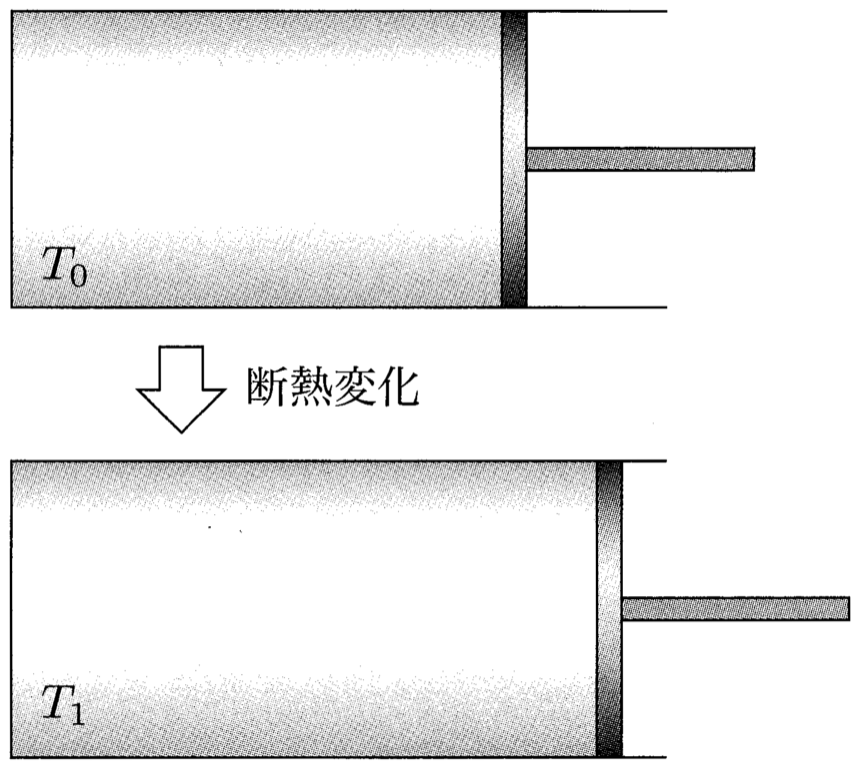
\includegraphics[keepaspectratio,width=50mm]{fig/ch17_ex13_cyl.png}
\end{zuright}
\hspace{1zw}この状態から外気圧をゆっくりと変化させ，気体の温度が$T_1\U{K}$($<T_0$)となるまで変化させた．理想気体が断熱変化するときは比熱比を$\gamma$として，ポアソンの式$PV^\gamma=（一定）$が成立することを用いてよい．気体定数を$R\U{J/mol\cdot K}$として以下の問に答えよ．
\begin{komon}
\ko{1} この状態変化を$P-V$図で表せ．ただし，終状態の体積を$V_1\U{m^3}$として図示せよ．
\ko{2} この気体が始状態から定温条件で体積$V_1\U{m^3}$となるまで変化した場合，気体はどのような曲線上を動くか．(1)の$P-V$図に点線で記入せよ．
\ko{3} この気体の内部エネルギー変化$\Delta U\U{J}$を求めよ．
\ko{4} この気体が外界にした仕事$w\U{J}$を求めよ．
\ko{5} 終状態における気体の体積$V_1\U{m^3}$を求めよ．
\end{komon}
\end{reidai}

\begin{sisinE}
温度が下がる断熱変化であるから，気体は外界に仕事をして膨張する（$V_1>V_0$）．$P-V$図では断熱曲線は等温曲線より急な右下がりの曲線になるので，同じ体積$V_1$まで変化させたとき断熱変化の方が圧力は低い．

断熱変化では$Q=0$なので，仕事$w$は積分せずとも熱力学第一法則$\Delta U=Q+(-w)$から求まる．体積を問われている(5)では，$P$と$V$を結ぶ$PV^\gamma=（一定）$ではなく$T$と$V$を結ぶ$TV^{\gamma-1}=（一定）$を使う．
\end{sisinE}

\Key{断熱変化中は比熱比$\gamma=\dfrac{C_P}{C_V}$を用いて $PV^\gamma=（一定）$, $TV^{\gamma-1}=（一定）$ が成立する}

\begin{kaitou}
\begin{komon}
\item[{\makebox[1.9zw][r]{(1)(2)}}] 断熱変化（実線）は$PV^\gamma=（一定）$，等温変化（点線）は$PV=（一定）$の曲線である．$\gamma>1$であるから断熱曲線の方が急になり，次図の通り．
       \begin{center}
       \ifbsAnaume
       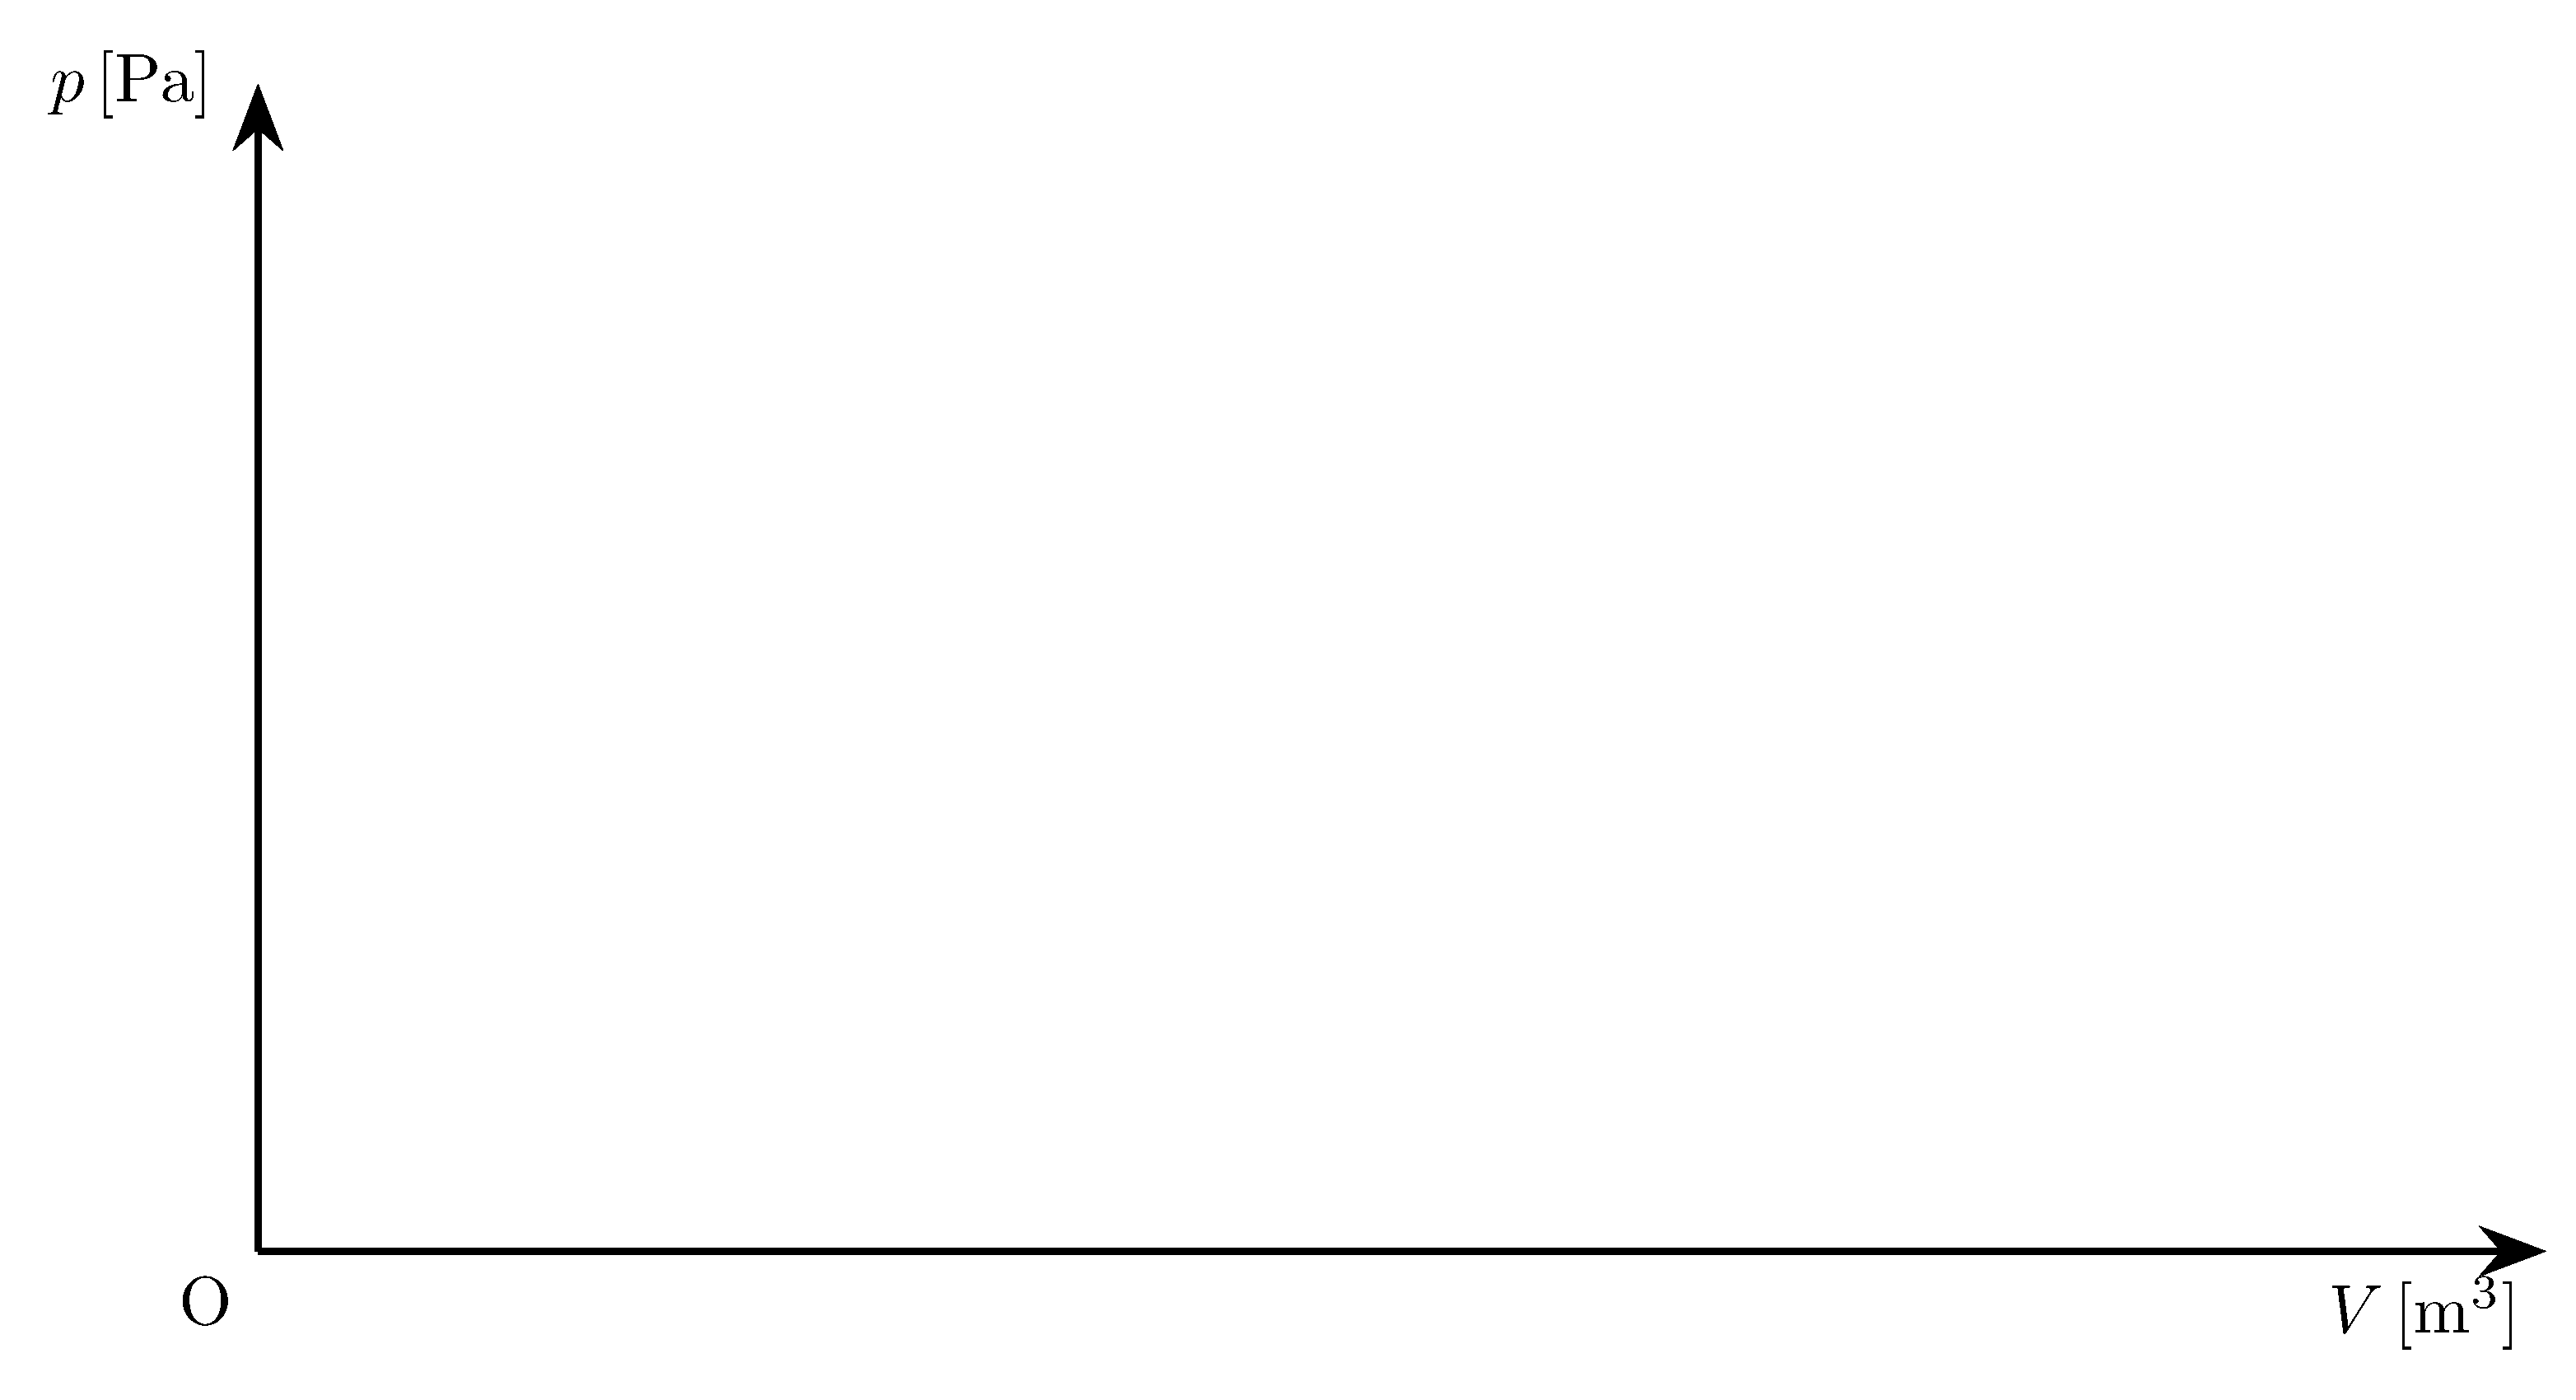
\includegraphics[keepaspectratio,width=106mm]{fig/ch17_ex13_pv_blank.png}
       \else
       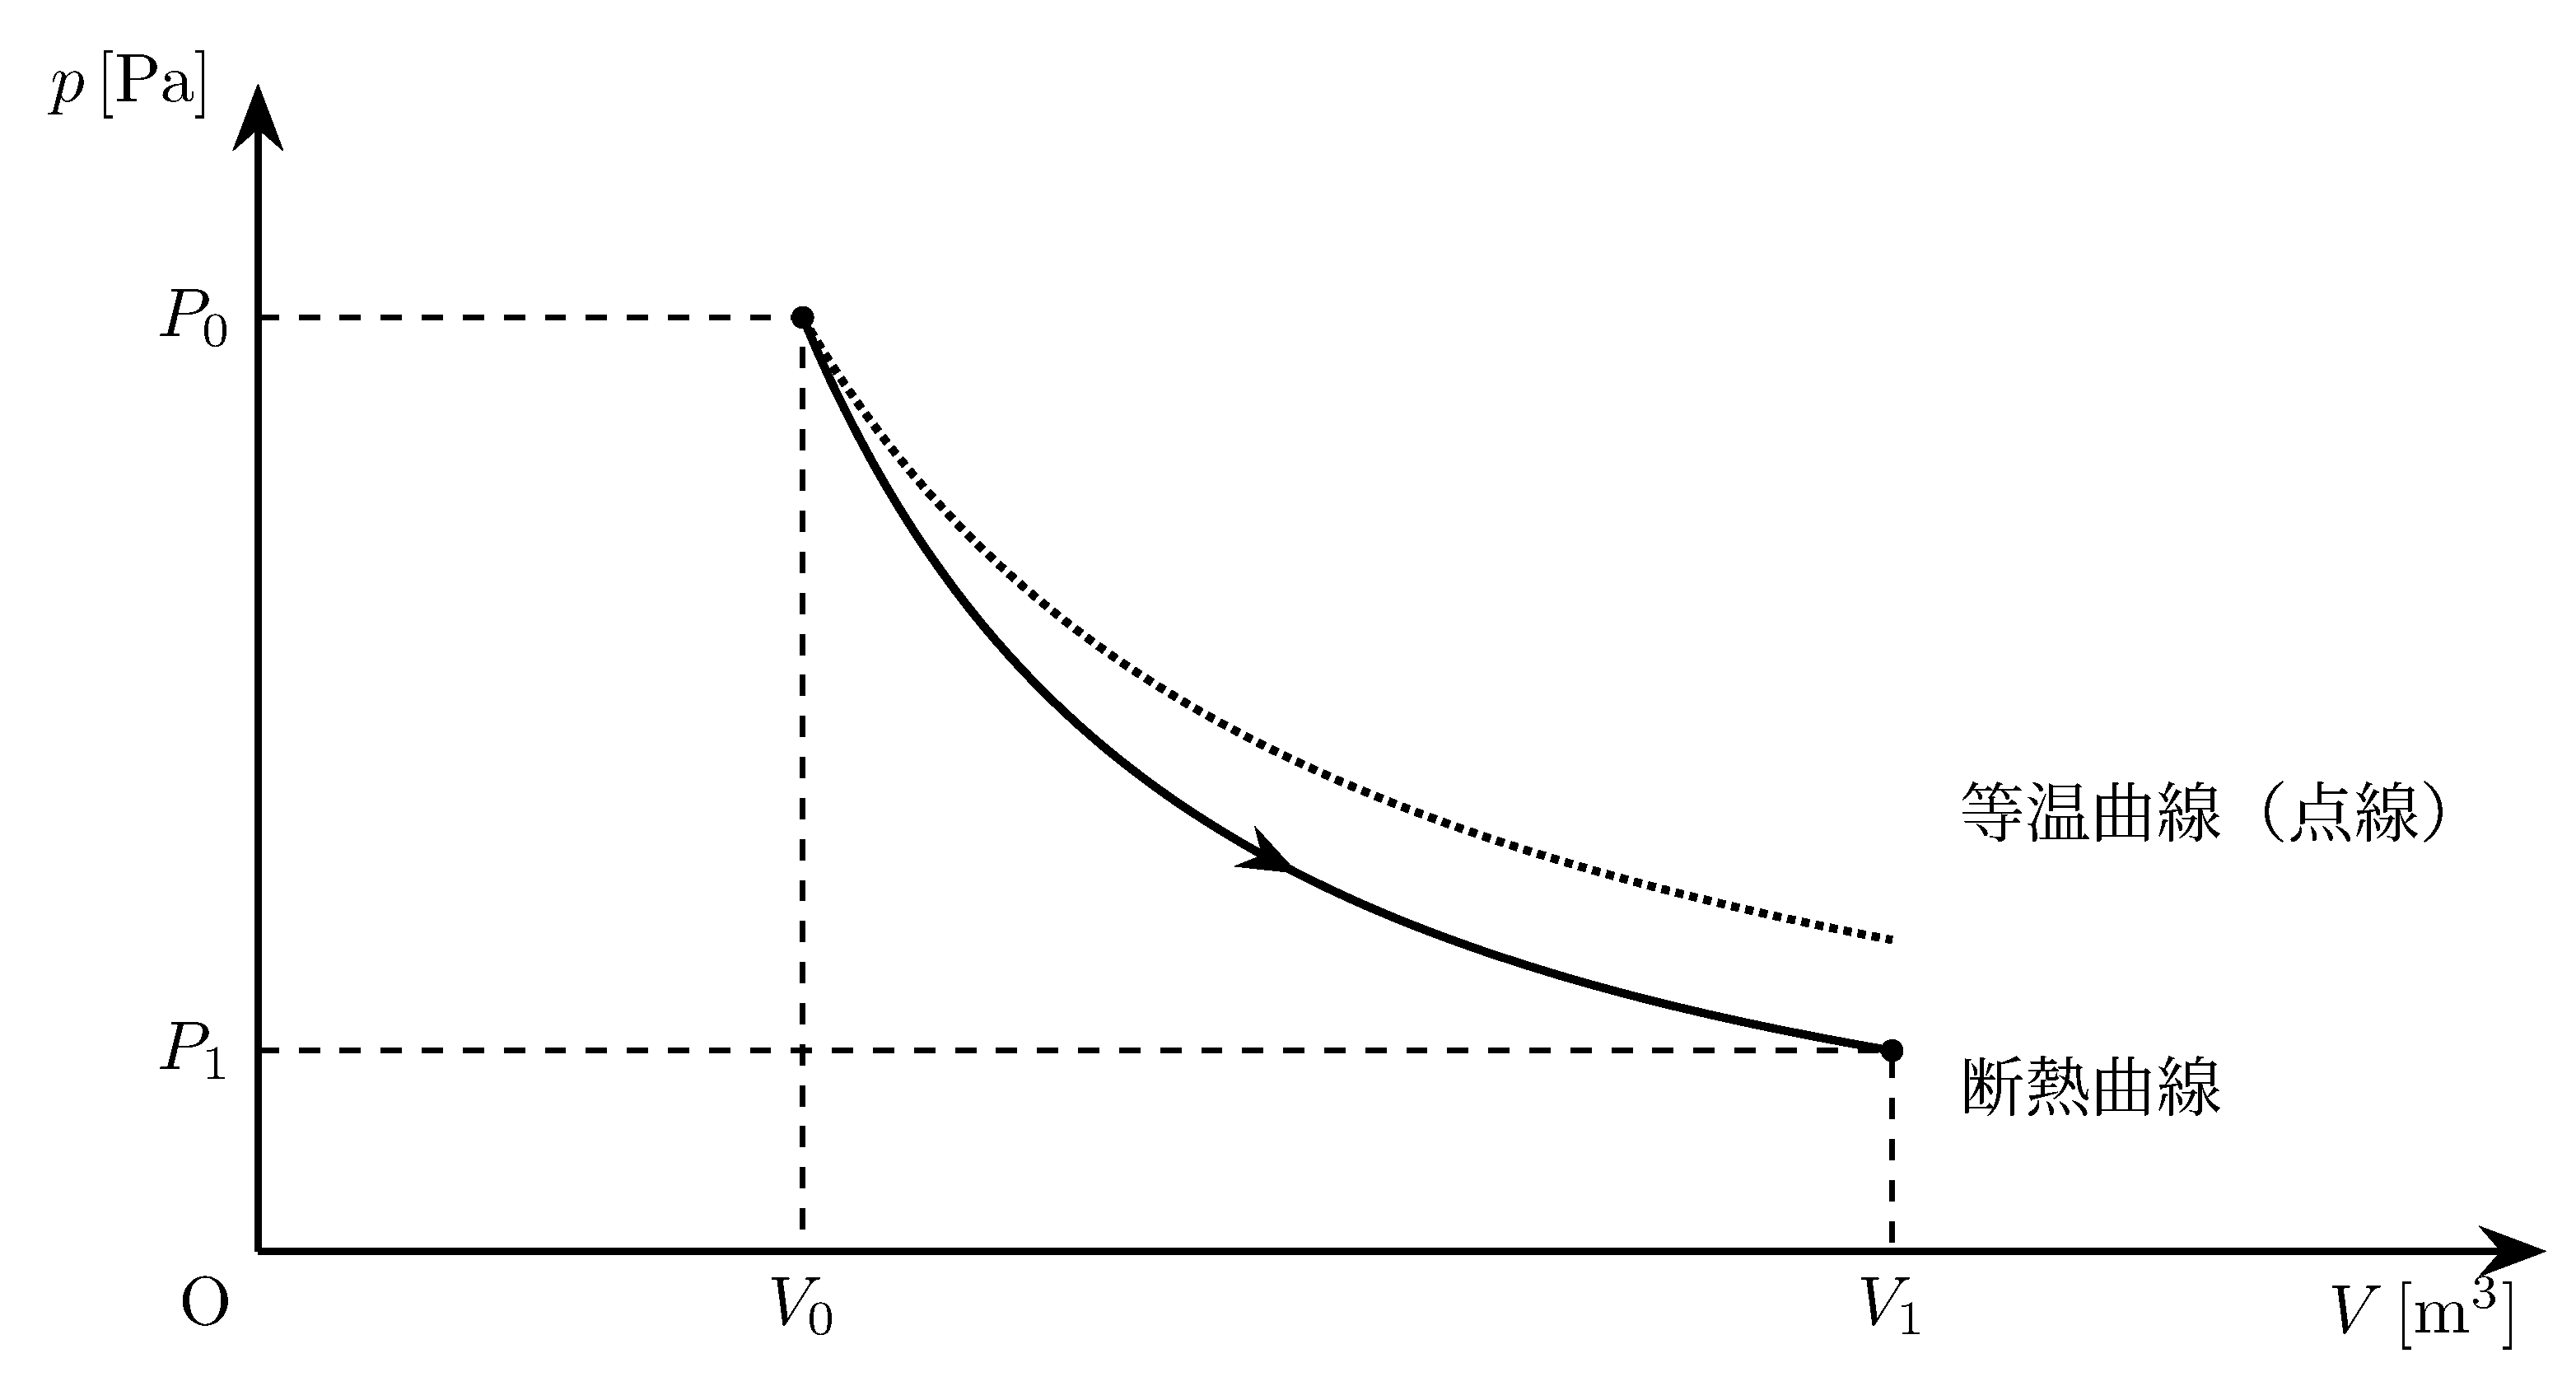
\includegraphics[keepaspectratio,width=106mm]{fig/ch17_ex13_pv.png}
       \fi
       \end{center}
       \hspace*{\fill}\Ans
\ko{3} 内部エネルギーは絶対温度だけで決まるので，
       \Ana{\Delta U=nC_V(T_1-T_0)\U{J}\Ans}
       $T_1<T_0$であるから$\Delta U<0$，すなわち内部エネルギーは減少する．
\ko{4} 断熱変化であるから$Q=0$であり，熱力学第一法則$\Delta U=Q+(-w)$より，
       \Ana{w=-\Delta U=nC_V(T_0-T_1)\U{J}\Ans}
\ko{5} マイヤーの関係式$C_P=C_V+R$より$\gamma-1=\dfrac{C_P}{C_V}-1=\dfrac{R}{C_V}$である．ポアソンの式\mbox{$TV^{\gamma-1}=（一定）$}を始状態と終状態に適用して，
       \[T_0V_0^{\gamma-1}=T_1V_1^{\gamma-1}\]
       これを$V_1$について解くと，
       \Ana{V_1=V_0\left(\frac{T_0}{T_1}\right)^{\frac{1}{\gamma-1}}
             =V_0\left(\frac{T_0}{T_1}\right)^{\frac{C_V}{R}}\U{m^3}\Ans}
       $T_0>T_1$であるから$V_1>V_0$となり，膨張していることが確かめられる．
\end{komon}
\end{kaitou}
\end{reidaiunit}


\subsection{自由膨張}
% 加筆（2026-09-02）：原本 p81 は「次の例題のように，」で始まり，例題14 を指している．
%   例題14 を原本と同じ位置（まとめ枠の直後）に入れたので，この言い回しを戻した．
次の例題のように，気体が真空中に拡散していく際には，左右の部屋の圧力が異なる状態を経て気体が真空側へと流れていき，最終的には両方の部屋の気体の圧力が等しくなったところで気体の流れが止まる．
このような真空中への気体の膨張を{\bf 自由膨張}といい，特に熱を遮断した状態で真空中へ膨張させることを{\bf 断熱自由膨張}という．

断熱自由膨張では，もともと気体の入っていた部屋から気体が出ていき，片方の部屋に注目すると気体のモル数が変化していくため，準静的な断熱変化で議論した場合と異なる．
そのため，断熱変化ではあるものの，ポアソンの式$PV^\gamma=（一定）$を用いて考えてはいけない．
このような場合は，箱全体に着目し熱力学第一法則を適用する．箱全体の体積は変わらず，また断熱変化なら箱の内外の熱のやりとりが0[J]である．
よって，箱内部の内部エネルギー変化が0[J]となることがわかる．

\begin{matome}{断熱自由膨張}
 \hspace{3mm} 熱を遮断した状態で真空中へ理想気体を膨張させるときは箱全体に対して熱力学第一法則を考える．
 \end{matome}

\begin{reidaiunit}
\begin{reidai}{断熱自由膨張}
\begin{zuright}{52mm}
\hspace{1zw}断熱材で作られた容器の中に，仕切板を隔てて図の左側の空間にのみ定積モル比熱が$C_V\U{J/mol\cdot K}$，温度が$T_0\U{K}$の理想気体が$n\U{mol}$封入されている．
\zusep
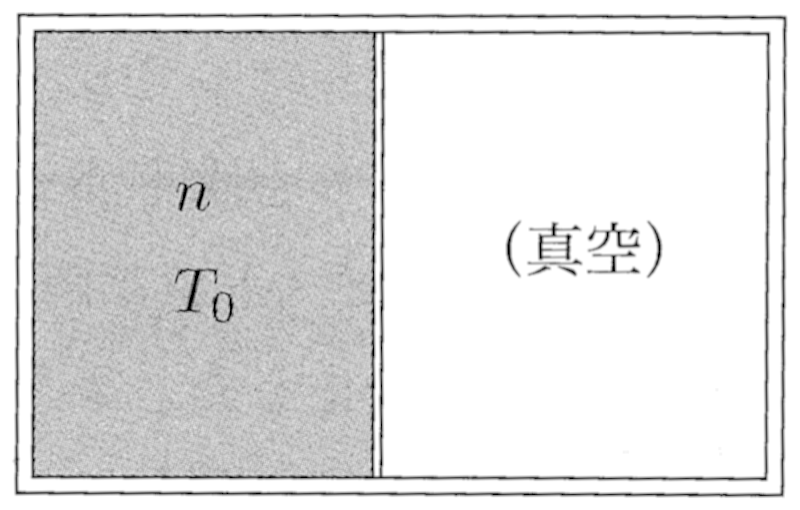
\includegraphics[keepaspectratio,width=52mm]{fig/ch17_ex14_box1.png}
\end{zuright}
\begin{komon}
\ko{1} この仕切板に穴を開けると気体は右側へと拡散していく．十分時間がたったのちの気体の温度$T^\prime\U{K}$を求めよ．
\end{komon}
\begin{zuright}{52mm}
\hspace{1zw}先と同じく断熱材で作られた容器の中に，仕切板を隔てて図のように左側，右側それぞれに異なる気体を封入する．左側（体積$V_1\U{m^3}$）には定積モル比熱$C_{V1}\U{J/mol\cdot K}$，温度が$T_1\U{K}$の理想気体が$n_1\U{mol}$だけ封入されており，右側（体積$V_2\U{m^3}$）には定積モル比熱$C_{V2}\U{J/mol\cdot K}$，温度が$T_2\U{K}$の理想気体が$n_2\U{mol}$だけ封入されている．
\zusep
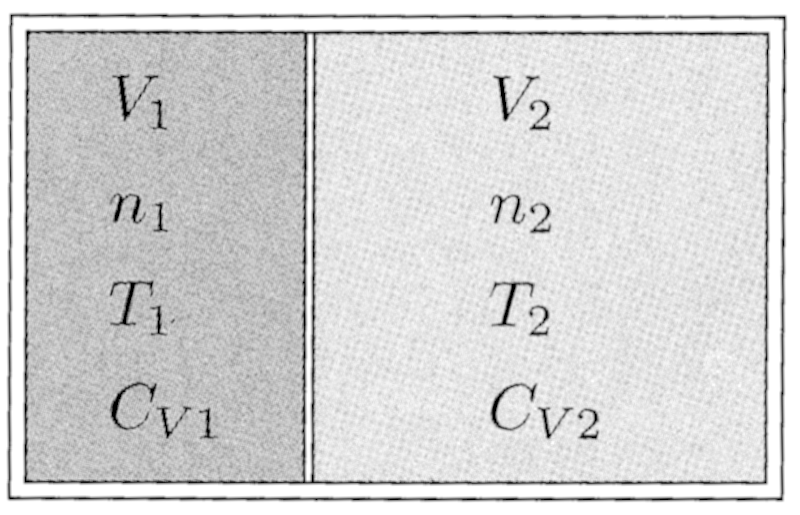
\includegraphics[keepaspectratio,width=52mm]{fig/ch17_ex14_box2.png}
\end{zuright}
\begin{komon}
\ko{2} この仕切板を取り外し，外界との熱のやり取りを断って2つの気体を混合する．十分時間がたったのちの温度$T\U{K}$を求めよ．
\end{komon}
\end{reidai}

\begin{sisinE}
どちらも{\gtfamily 容器全体を一つの系とみなして熱力学第一法則を立てる}．容器の体積は変わらないので外界と仕事のやり取りはなく（$W=0$），断熱材で作られているので熱のやり取りもない（$Q=0$）．したがって容器全体の内部エネルギーの変化は$\Delta U=0$である．

(2)では，容器全体の内部エネルギー変化は左側の気体の変化と右側の気体の変化の和であることを使う．
\end{sisinE}

\Key{真空中への断熱自由膨張 $\Rightarrow$ 箱全体に対しての熱力学第一法則}

\begin{kaitou}
\begin{komon}
\ko{1} 容器全体を一つの系とみなすと，体積が変わらないので$W=0$，断熱材なので$Q=0$である．よって熱力学第一法則より
       \[\Delta U=Q+W=0\]
       一方，内部エネルギーの変化は$\Delta U=nC_V(T^\prime-T_0)$と表せるから，$nC_V\neq 0$より$T^\prime-T_0=0$，すなわち
       \Ana{T^\prime=T_0\U{K}\Ans}
\ko{2} こちらも容器全体では$Q=0$, $W=0$であるから$\Delta U=0$である．混合後の温度を$T\U{K}$とすると，左側の気体の内部エネルギー変化と右側の気体の内部エネルギー変化の和が$\Delta U$であるから，
       \[n_1C_{V1}(T-T_1)+n_2C_{V2}(T-T_2)=0\]
       これを$T$について解いて，
       \Ana{T=\frac{n_1C_{V1}T_1+n_2C_{V2}T_2}{n_1C_{V1}+n_2C_{V2}}\U{K}\Ans}
\end{komon}
\end{kaitou}
\end{reidaiunit}



\newpage

%%%%%%%%%%%%%%%%%%%%  練習問題（旧 prob_p43.png / prob_p44.png / prob_p45.png）  %%%%%%%%%%%%%%%%%%%%
% 第16回の［23］に続く．章単体で組んだときも番号が本体と一致するように明示しておく
\setcounter{qno}{23}

\filbreak
\Rank{A問題}

\Mon{基本事項の確認}

\hspace{1zw}以下の設問に答えよ．

\hspace{1zw}単原子分子理想気体，二原子分子理想気体の定積モル比熱はそれぞれ$\dfrac{3}{2}R$, $\dfrac{5}{2}R$である．このときそれぞれの比熱比はいくらか．

\filbreak
\Rank{B問題}

\Mon{状態変化に伴う各物理量の変化}

\hspace{1zw}ピストンのついた容器の中に一定量の気体を入れ，次の各変化を行う場合，\MARU{1}\MARU{2}\MARU{3}\MARU{4}に適するものを選べ．
\begin{komon}
\ko{1} 圧力を一定に保って圧縮させるとき
\ko{2} 体積を一定に保って減圧するとき
\ko{3} 温度を一定に保って加圧するとき
\ko{4} 外界との熱のやり取りを断ち切って圧縮するとき
\end{komon}
\hspace{1zw}各状態変化において，
\begin{list}{}{\setlength{\leftmargin}{2zw}\setlength{\itemsep}{0.4mm}\setlength{\topsep}{0.6mm}\setlength{\parsep}{0pt}}
\item[・] 外界が気体に与える熱量$Q$は，\fbox{\MARU{1}：正，\,0，\,負}となる．
\item[・] 外界が気体に対してする仕事$W$は，\fbox{\MARU{2}：正，\,0，\,負}となる．
\item[・] 気体の内部エネルギーの変化量$\Delta U$は，\fbox{\MARU{3}：正，\,0，\,負}となる．
\item[・] 気体の温度は，\fbox{\MARU{4}：上昇する，一定である，下降する}．
\end{list}

\Mon{定温変化}

\begin{zuright}{58mm}
\hspace{1zw}右図のように断面積$S\U{m^2}$のシリンダーの中に，ピストンで定積モル比熱が$C_V\U{J/mol\cdot K}$の理想気体を$n\U{mol}$だけ封入した．ピストンは軽くて自由に動くことができ，棒が取り付けられてある．
\zusep
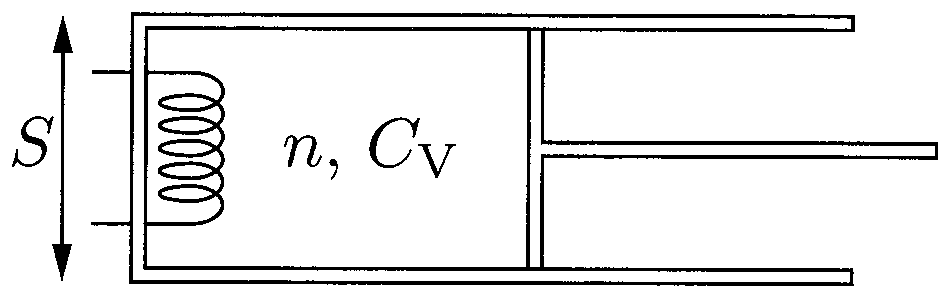
\includegraphics[keepaspectratio,width=58mm]{fig/ch17_p43_cyl.png}
\end{zuright}
\hspace{1zw}初め，シリンダーの底からピストンまでの距離は$l_0\U{m}$であり，また気体の温度は$T_0\U{K}$であった．シリンダー内にはヒーターが取り付けられており，気体に対して熱を与えることができる．シリンダーおよびピストンは断熱材でできており，ヒーターによって与えた熱が大気に拡散することはないものとする．気体定数を$R\U{J/mol\cdot K}$として以下の設問に答えよ．
\begin{komon}
\ko{1} 初めの状態におけるシリンダー内の気体の圧力$p_0\U{Pa}$を求めよ．
\end{komon}
\hspace{1zw}ここで，気体が温度$T_0\U{K}$を保つようにピストンを操作しながら内部の気体をヒーターでゆっくりと加熱したところ，ピストンはゆっくりと移動し，シリンダーの底からピストンまでの距離が$l_1\U{m}$となったところで加熱をやめた．
\begin{komon}
\ko{2} 終状態における気体の圧力$p_1\U{Pa}$を求めよ．
\ko{3} この変化において，気体が外界にした仕事$w\U{J}$を求めよ．
\ko{4} ヒーターによって加えた熱量$Q\U{J}$を求めよ．
\end{komon}

\Mon[\Sitei]{断熱変化}

\begin{zuright}{58mm}
\hspace{1zw}右図のように断面積$S\U{m^2}$のシリンダーの中に，ピストンで定積モル比熱が$C_V\U{J/mol\cdot K}$の理想気体を$n\U{mol}$だけ封入した．ピストンは軽くて自由に動くことができ，棒が取り付けられてある．
\zusep
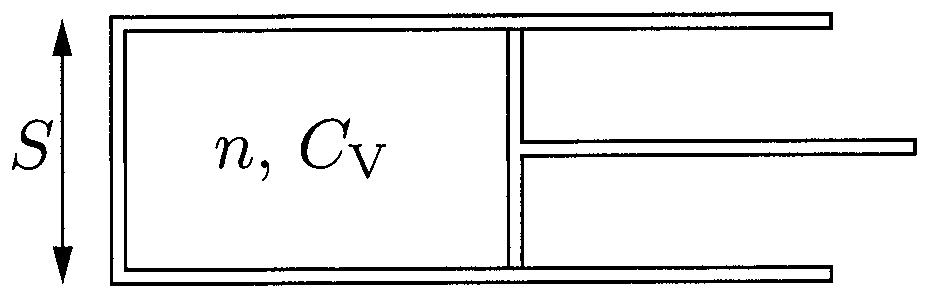
\includegraphics[keepaspectratio,width=58mm]{fig/ch17_p44_cyl.png}
\end{zuright}
\hspace{1zw}シリンダーおよびピストンは断熱材でできており，外界と熱のやり取りはない．棒を手で持って動かし，シリンダーの底からピストンまでの距離が$l_0\U{m}$となる位置に持ってきたところ気体の温度は$T_0\U{K}$となった．気体定数を$R\U{J/mol\cdot K}$として以下の設問に答えよ．
\begin{komon}
\ko{1} この状態におけるシリンダー内の圧力$p_0\U{Pa}$を求めよ．
\end{komon}
\hspace{1zw}ここでピストンを手でゆっくりと引き，シリンダーの底からピストンまでの距離が$l_1\U{m}$になるまで気体を膨張させた．
\begin{komon}
\ko{2} ポアソンの法則を用いて，終状態における気体の圧力$p_1\U{Pa}$および温度$T_1\U{K}$を求めよ．
% 誤植訂正（2026-09-02）：原本は「温度 T_1[K] 求めよ」で助詞「を」が欠けていた．
\ko{3} この状態変化を$p-V$図で表せ．
\ko{4} この変化において，気体が外界にした仕事$w\U{J}$を求めよ．
\end{komon}

\Mon{断熱自由膨張}

\begin{zuright}{56mm}
\hspace{1zw}右図のように，体積$V_\mathrm{A}\U{m^3}$, $V_\mathrm{B}\U{m^3}$の断熱容器A，Bをコックのついた細い管でつないである．はじめコックは閉じられており，Aだけに定積モル比熱$C_V\U{J/mol\cdot K}$の理想気体が圧力$p_0\U{Pa}$，温度$T_0\U{K}$となって入っている．コックを開いたところ気体はBへと拡散していき，十分時間が経つと全体が一様となった．このときA，B内の気体の圧力および温度を求めよ．ただし，気体定数を$R\U{J/mol\cdot K}$とする．
\zusep
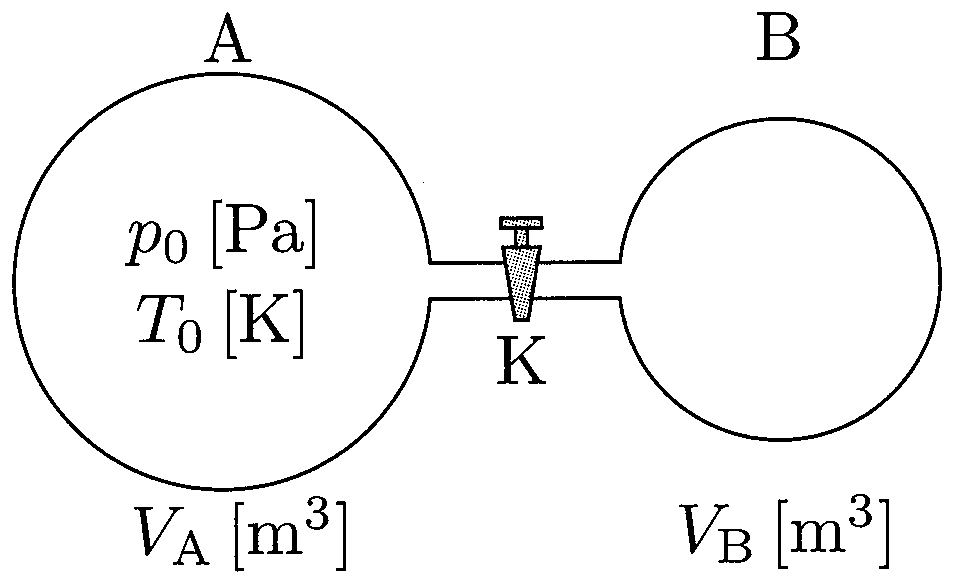
\includegraphics[keepaspectratio,width=56mm]{fig/ch17_p44_ab.png}
\end{zuright}

\Mon[\Sitei]{断熱膨張・断熱自由膨張}

\begin{zuright}{56mm}
\hspace{1zw}右図のようにバルブつきの隔壁で仕切られたシリンダーがある．隔壁の左側の体積は$V_0\U{m^3}$であり，ここに定積モル比熱$C_V\U{J/mol\cdot K}$の理想気体が圧力$p_0\U{Pa}$，温度$T_0\U{K}$となって封入されている．
\zusep
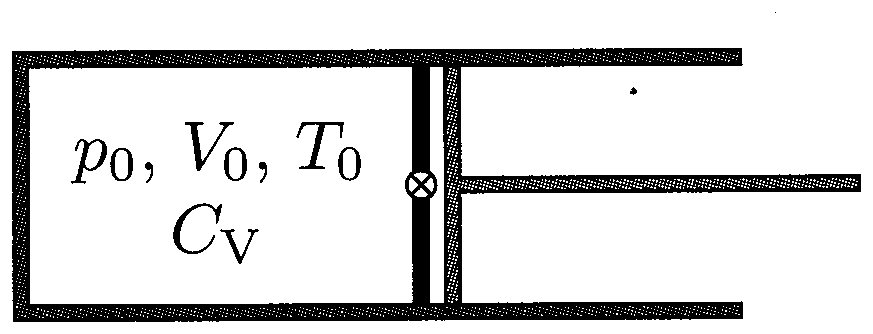
\includegraphics[keepaspectratio,width=56mm]{fig/ch17_p44_valve.png}
\end{zuright}
\hspace{1zw}隔壁の右側は取っ手付きのピストンが取り付けられている．初めバルブは閉じており，右側の空間には気体は封入されておらず，ピストンは隔壁に接触して体積が0になっている．シリンダー，ピストン，隔壁，バルブなどはすべて断熱材で出来ており，外界との熱のやり取りはない．

\hspace{1zw}この状態から以下の二つの方法によって左側に封入されている気体を右側に拡散させる．このとき，終状態における気体の圧力および温度をそれぞれ求めよ．気体定数を$R\U{J/mol\cdot K}$とする．
\begin{komon}
\ko{1} バルブを閉じたまま取っ手を引いて右側に体積$V_0\U{m^3}$の真空を作ったのち，バルブを全開にして気体を右側へ拡散させる．
\ko{2} バルブを全開にしてから取っ手をゆっくりと引き，右側の空間の体積を少しずつ増加させて体積$V_0\U{m^3}$にする．
\end{komon}

\filbreak
\Rank{C問題}

\Mon{気体の一般的な状態変化}

\begin{zuright}{62mm}
\hspace{1zw}図のように断面積$S\U{m^2}$のシリンダーに定積モル比熱が$C_V\U{J/mol\cdot K}$の理想気体を封入し，ピストンに図のように弾性定数が$k\U{N/m}$のバネを取り付けた．バネが自然長のとき，ちょうど大気圧$P_0\U{Pa}$とシリンダー内の気体の圧力とがつり合い，このときの気体の温度は$T_0\U{K}$，気柱の長さは$l_0\U{m}$であった．
\zusep
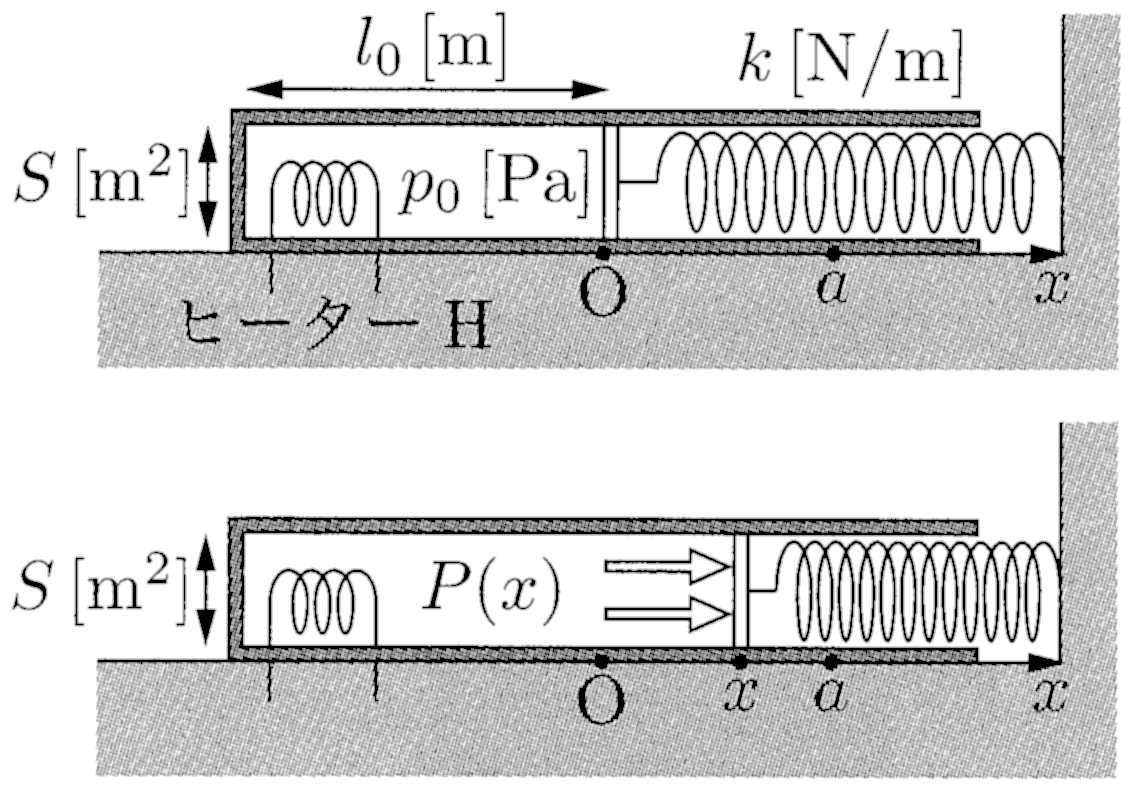
\includegraphics[keepaspectratio,width=62mm]{fig/ch17_p45_spring.png}
\end{zuright}
\hspace{1zw}シリンダー内のヒーターHから少しずつ気体を加熱していったところ，気体はゆっくりと膨張し，ピストンはゆっくりと距離$a\U{m}$だけ進んだ．シリンダー，容器などはすべて断熱材で出来ており，バネなどの熱容量は無視してよい．気体定数を$R\U{J/mol\cdot K}$として以下の設問に答えよ．
\begin{komon}
\ko{1} 終状態における気体の圧力$P_1\U{Pa}$および温度$T_1\U{K}$を求めよ．
\ko{2} この状態変化で気体がする仕事$w\U{J}$を求めよ．
\ko{3} この状態変化で気体に与えた熱量$Q\U{J}$を求めよ．
\end{komon}

\newpage

%%%%%%%%%%%%%%%%%%%%  解答（旧 prob_p132.png 〜 prob_p136_1.png）  %%%%%%%%%%%%%%%%%%%%
\KaiTitle{第17回　気体の状態変化\MARU{2}}
\setlength{\columnseprule}{0.4pt}
\begin{multicols}{2}
\raggedcolumns

\Rank{A問題}
\MonN{24}{基本事項の確認}\par\nopagebreak
\begin{sisin}
比熱比の定義式$\gamma=\dfrac{C_P}{C_V}$とマイヤーの関係式$C_P=C_V+R$を利用する．比熱比の分母・分子がどちらにくるかは，\underline{比熱比は}\hskip0pt\underline{必ず$1$}\hskip0pt\underline{より大}\hskip0pt\underline{きい}と覚えておけば間違いがない．
\end{sisin}
\KaiHead
マイヤーの関係式$C_P=C_V+R$を用いると，
\[\gamma=\frac{C_P}{C_V}=1+\frac{R}{C_V}\]
であるから，
\[\text{単原子分子理想気体：}\gamma=1+\frac{R}{\frac{3}{2}R}=\frac{5}{3}\]
\[\text{二原子分子理想気体：}\gamma=1+\frac{R}{\frac{5}{2}R}=\frac{7}{5}\Ans\]

\Rank{B問題}
\MonN{25}{状態変化に伴う各物理量の変化}\par\nopagebreak
\begin{sisin}
各状態変化で，熱量，仕事，内部エネルギーのどれが$0$になるのか（もしくは特殊な値・式となるのか）を覚えておき，残りの量については，$-W=\displaystyle\int_{V_{\mathrm{initial}}}^{V_{\mathrm{final}}}P(V)dV$, $\Delta U=nC_V\Delta T$, $\Delta U=Q+W$の各式から正負を判定する．

状態変化前後の状態方程式の両辺を差し引くと，
\[\begin{array}{r@{\;}l}
       & P_1V_1=nRT_1\\
 -)\;\;& P_0V_0=nRT_0\\ \hline
       & P_1V_1-P_0V_0=nR(T_1-T_0)
\end{array}\]
となる．ここで$PV$の項の変化$P_1V_1-P_0V_0$を$\Delta(PV)$と書くと，
\[\Delta(PV)=nR\cdot\Delta T\]
がすべての状態変化に対して成立する．温度変化についてはこれを利用して考えると便利である．
\end{sisin}
\KaiHead
状態変化前を$(P_0,V_0,T_0)$，変化後を$(P_1,V_1,T_1)$とする．$W$は外部が気体に対してした仕事であるから，気体が外部に対してした仕事は$(-W)$で表され，$-W=\displaystyle\int_{V_{\mathrm{initial}}}^{V_{\mathrm{final}}}P(V)dV$が成り立つ．内部エネルギーは絶対温度にのみ依存し$\Delta U=nC_V\Delta T$と表せる．また，熱力学の第一法則より$\Delta U=Q+W$，変化前後の状態方程式を辺々引いて，$P_1V_1-P_0V_0=nR(T_1-T_0)$が成り立つ．体積変化$\Delta V$を$\Delta V=V_1-V_0$とする．
\begin{komon}
\ko{1} 定圧であるから，$-W=P_0\cdot\Delta V$と表せる．\par
       \hspace*{1zw}圧縮しているので$\Delta V<0$であるから$W>0$，また$P_0\cdot\Delta V<0$であるから温度変化は$\Delta T<0$である．よって$\Delta U<0$となり，$Q=\Delta U+(-W)<0$である．
       \[\text{\MARU{1}負，\MARU{2}正，\MARU{3}負，\MARU{4}下降する}\Ans\]
\ko{2} 定積であるから$\Delta V=0$であり，$W=0$である．\par
       \hspace*{1zw}減圧していくので，$P_1V_0-P_0V_0<0$であるから温度変化は$\Delta T<0$である．よって$\Delta U<0$となり，$Q=\Delta U+(-W)<0$である．以上より，
       \[\text{\MARU{1}負，\MARU{2}$0$，\MARU{3}負，\MARU{4}下降する}\Ans\]
\ko{3} 定温であるから温度が一定であり，$\Delta U=0$である．\par
       \hspace*{1zw}加圧しているので$P_1>P_0$であり，状態方程式$P_1V_1=nRT_0$および$P_0V_0=nRT_0$より$V_1<V_0$, すなわち体積は減少している．よって$W>0$であり，$Q=\Delta U+(-W)<0$である．以上より，
       \[\text{\MARU{1}負，\MARU{2}正，\MARU{3}$0$，\MARU{4}一定である}\Ans\]
       \begin{chuu}
       気体が外部にした仕事$(-W)$の正負は$P-V$図から考えれば明らかである．定温曲線は次図のように双曲線となるのだから，加圧すれば体積は減少する．よって，$-W<0$となるのはこの図より明らか．
       % 誤植訂正（2026-09-02）：原本は「よって，W<0 となるのは…」．
       %   直前で「気体が外部にした仕事 (-W) の正負は」と述べており，加圧＝圧縮
       %   では (-W)<0（したがって W>0）．本解の(3)も「よって W>0 であり」と
       %   しているので，(-W)<0 に改めた．
       \begin{center}
       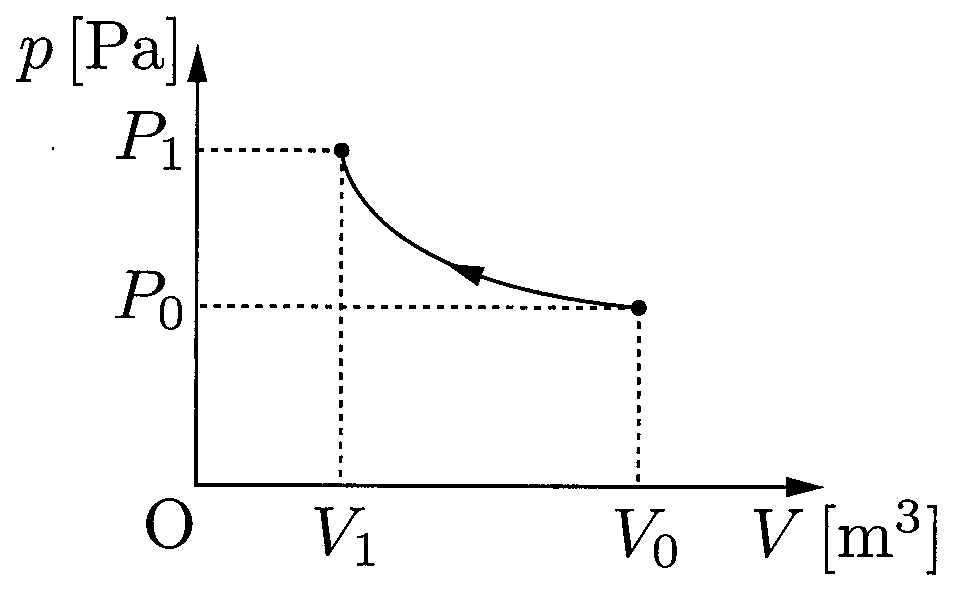
\includegraphics[keepaspectratio,width=54mm]{fig/ch17_a25_pv.png}
       \end{center}
       \end{chuu}
\ko{4} 断熱変化であるから，$Q=0$である．\par
       \hspace*{1zw}圧縮しているので$\Delta V<0$であるから$W>0$，また$\Delta U=Q+W$より$\Delta U>0$であるから温度変化は$\Delta T>0$である．以上より，
       \[\text{\MARU{1}$0$，\MARU{2}正，\MARU{3}正，\MARU{4}上昇する}\Ans\]
       \begin{chuu}
       (1)〜(4)の各状態変化ごとに本質的に覚えておくべきことは最初の一行のみである．あとは指針で述べた関係式から他の物理量の変化が分かる．
       \end{chuu}
\end{komon}

\MonN{26}{定温変化}\par\nopagebreak
\begin{sisin}
本問のように，変化途中で気体の圧力が変化する場合には$w=P\cdot\Delta V$としてはいけない．体積が$V\U{m^3}$のときの圧力$P(V)\U{Pa}$を求め，これを積分することで求める．
\end{sisin}
\KaiHead
\begin{komon}
\ko{1} 最初の状態について状態方程式を立てると，
       \[p_0\cdot Sl_0=nRT_0\]
       であるから，
       \[p_0=\frac{nRT_0}{Sl_0}\U{Pa}\Ans\]
\ko{2} 終状態における状態方程式は，
       \[p_1\cdot Sl_1=nRT_0\]
       であるから，
       \[p_1=\frac{nRT_0}{Sl_1}\U{Pa}\Ans\]
\ko{3} 気体の体積が$V\U{m^3}$のときの気体の圧力を$p(V)\U{Pa}$とし，このときの気体の状態方程式を立てると，
       \[p(V)\cdot V=nRT_0\]
       これより，
       \[p(V)=\frac{nRT_0}{V}\]
       よって，体積が$V=Sl_0\rightarrow Sl_1\U{m^3}$に変化するまでに気体が外部にした仕事$w$は，$nRT_0$が定数であることに注意して
       \[\begin{aligned}
         w&=\int_{Sl_0}^{Sl_1}p(V)dV=\int_{Sl_0}^{Sl_1}\frac{nRT_0}{V}dV\\
          &=nRT_0\int_{Sl_0}^{Sl_1}\frac{1}{V}dV\\
          &=nRT_0\Bigl[\log_e|V|\Bigr]_{Sl_0}^{Sl_1}\\
          &=nRT_0\log_e\frac{l_1}{l_0}\U{J}\Ans
       \end{aligned}\]
\ko{4} この状態変化にて気体の温度は$T_0$一定であるから，気体の内部エネルギー変化$\Delta U\U{J}$は
       \[\Delta U=nC_V\Delta T=0\]
       である．熱力学第一法則より$Q$, $\Delta U$, $w$の間には，
       \[\Delta U=Q+(-w)\]
       の関係が成り立つ．以上より気体に加えた熱量は
       \[Q=nRT_0\log_e\frac{l_1}{l_0}\U{J}\Ans\]
\end{komon}

\MonN{27}{断熱変化}\par\nopagebreak
\begin{sisin}
ピストンはゆっくりと移動するので，この状態変化は準静的過程である．理想気体の均一系準静的断熱変化では，ポアソンの式
\[PV^\gamma=（一定）,\;TV^{\gamma-1}=（一定）\]
が成立する．どちらの式を利用した方がよいかは問題文に与えられている文字で考えよ．本問では$p$, $T$の両方が問われているのでどちらを利用してもよい．前者の$pV^\gamma=（一定）$で考えた場合を示す．

断熱曲線の勾配は等温曲線よりも急になる．

\underline{断熱変化の}\hskip0pt\underline{場合に限}\hskip0pt\underline{り，$w$を}\hskip0pt\underline{熱力学第}\hskip0pt\underline{一法則か}\hskip0pt\underline{ら求める}\hskip0pt\underline{ことがで}\hskip0pt\underline{きる}．断熱変化の場合は$Q=0$であるから，$\Delta U$から$w$を求めることができるのである．もちろん$w=\displaystyle\int_{V_{\mathrm{initial}}}^{V_{\mathrm{final}}}P(V)dV$から求めることも可能である．
\end{sisin}
\KaiHead
気体の比熱比$\gamma$は，マイヤーの関係式を用いて，
\[\gamma=\frac{C_P}{C_V}=\frac{C_V+R}{C_V}=1+\frac{R}{C_V}\]
で与えられる．
\begin{komon}
\ko{1} 初めの状態について状態方程式を立てると，
       \[p_0Sl_0=nRT_0\]
       これを解いて，
       \[p_0=\frac{nRT_0}{Sl_0}\U{Pa}\Ans\]
\ko{2} 気体は外界と熱のやり取りをしておらず，断熱変化であるので，初状態と終状態に対してポアソンの式より，
       \[p_0(Sl_0)^\gamma=p_1(Sl_1)^\gamma\]
       が成り立つ．これを解いて，
       \[p_1=\frac{nRT_0}{Sl_0}\left(\frac{l_0}{l_1}\right)^{1+\frac{R}{C_V}}\U{Pa}\Ans\]
       また，終状態の状態方程式は，
       \[p_1Sl_1=nRT_1\]
       であるから，これを解いて
       \[T_1=T_0\left(\frac{l_0}{l_1}\right)^{\frac{R}{C_V}}\U{K}\Ans\]
       \begin{bekkai}
       もう一つのポアソンの式$TV^{\gamma-1}=$一定を利用してもよい．この場合は，
       \[T_0(Sl_0)^{\gamma-1}=T_1(Sl_1)^{\gamma-1}\]
       より，$T_1=T_0\left(\dfrac{l_0}{l_1}\right)^{\frac{R}{C_V}}\U{K}$を導くことができる．また，この$T_1$を元に終状態の状態方程式$p_1Sl_1=nRT_1$を立てて圧力$p_1$を求めることが可能である．

       ポアソンの式は多少面倒な式であるから，まず$pV^\gamma=$一定もしくは$TV^{\gamma-1}=$一定を用いて変化後の$p$, $T$のいずれか一方を求め，もう片方については状態方程式から求めればよい．両方をポアソンの式から求めるのは面倒なだけである．
       \end{bekkai}
\ko{3} 気体の体積が$V\U{m^3}$のときの気体の圧力を$p(V)\U{Pa}$とし，初状態とこの状態との間にポアソンの式より，
       \[p(V)V^\gamma=p_0(Sl_0)^\gamma\quad(=\text{一定})\]
       が成り立つ．よって，
       \[p(V)=p_0(Sl_0)^\gamma\frac{1}{V^\gamma}\]
       である．ここで$\gamma>1$に注意すると，これは右下がりの曲線を表すので，状態変化の$p-V$図は次図の通り．
       \begin{center}
       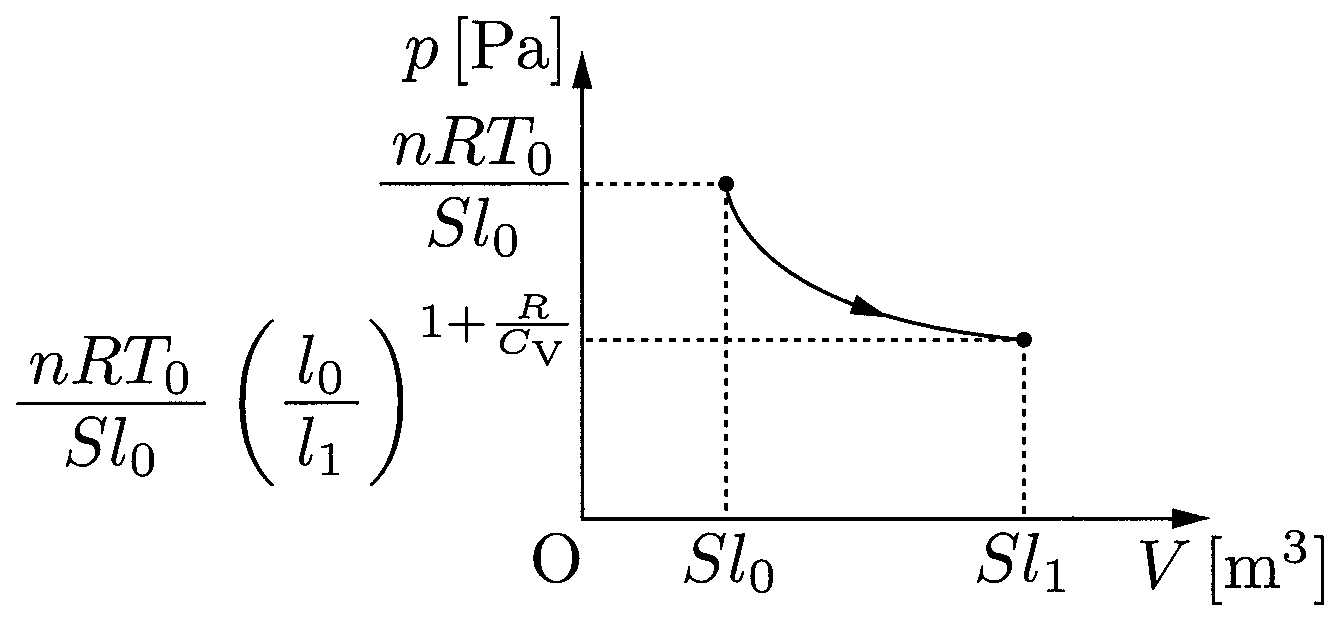
\includegraphics[keepaspectratio,width=64mm]{fig/ch17_a27_pv.png}
       \end{center}
       \hspace*{\fill}\Ans
\ko{4} この変化は断熱変化であるから，外部が気体に与える熱量$Q$は，
       \[Q=0\]
       また，この状態変化の内部エネルギーの増加量$\Delta U$は，
       \[\begin{aligned}
         \Delta U&=nC_V(T_1-T_0)\\
                 &=nC_VT_0\left\{\left(\frac{l_0}{l_1}\right)^{\frac{R}{C_V}}-1\right\}\U{J}
       \end{aligned}\]
       気体が外界に対してした仕事$w$は，熱力学第一法則を用いると，
       \[\Delta U=Q+(-w)\]
       の関係があるので，
       \[\begin{aligned}
         w&=-\Delta U\\
          &=nC_VT_0\left\{1-\left(\frac{l_0}{l_1}\right)^{\frac{R}{C_V}}\right\}\U{J}\Ans
       \end{aligned}\]
       \begin{bekkai}
       指針でも述べたように，まともに
       \[w=\int_{V_{\mathrm{initial}}}^{V_{\mathrm{final}}}P(V)dV\]
       を計算しても同一の答えが求められる．気体の体積が$V\U{m^3}$のときの気体の圧力$p(V)\U{Pa}$は，
       \[p(V)=p_0(Sl_0)^\gamma\frac{1}{V^\gamma}\]
       であるから，
       \[\begin{aligned}
         w&=\int_{Sl_0}^{Sl_1}p(V)dV\\
          &=p_0(Sl_0)^\gamma\int_{Sl_0}^{Sl_1}\frac{1}{V^\gamma}dV\\
          &=p_0(Sl_0)^\gamma\left[\frac{1}{-\gamma+1}V^{-\gamma+1}\right]_{Sl_0}^{Sl_1}\\
          &=p_0(Sl_0)^\gamma\left[-\frac{C_V}{R}\cdot\frac{1}{V^{\gamma-1}}\right]_{Sl_0}^{Sl_1}\\
          &=-\frac{C_V}{R}p_0(Sl_0)^{\gamma-1}(Sl_0)\\
          &\qquad\times\left\{\frac{1}{(Sl_1)^{\gamma-1}}-\frac{1}{(Sl_0)^{\gamma-1}}\right\}\\
          &=-\frac{C_V}{R}p_0(Sl_0)\left\{\left(\frac{l_0}{l_1}\right)^{\gamma-1}-1\right\}\\
          &=\frac{C_V}{R}\frac{nRT_0}{Sl_0}Sl_0\left\{1-\left(\frac{l_0}{l_1}\right)^{\frac{R}{C_V}}\right\}\\
          &=nC_VT_0\left\{1-\left(\frac{l_0}{l_1}\right)^{\frac{R}{C_V}}\right\}\U{J}
       \end{aligned}\]
       となり，全く同じ答えが導ける．しかし，この計算はなかなかに厄介である．断熱変化に限っては熱力学第一法則から$w$を求めることを覚えておくとよい．
       \end{bekkai}
\end{komon}

\MonN{28}{断熱自由膨張}\par\nopagebreak
\begin{sisin}
本問のような断熱自由膨張では，\underline{容器$\mathrm{A+B}$}\hskip0pt\underline{全体を一}\hskip0pt\underline{つの系と}\hskip0pt\underline{みなして}\hskip0pt\underline{熱力学第}\hskip0pt\underline{一法則を}\hskip0pt\underline{立てる}のがポイント．$\mathrm{A+B}$の全体積は$V_\mathrm{A}+V_\mathrm{B}\U{m^3}$のまま不変であるから，$\mathrm{A+B}$は容器外と仕事のやり取りをしない．また，断熱容器を使っているから熱のやり取りもない．以上に着目して熱力学第一法則を立てる．
\end{sisin}
\KaiHead
変化後の$\mathrm{A}$, $\mathrm{B}$内の気体の圧力を$p\U{Pa}$, 温度を$T\U{K}$とする．この変化において，$\mathrm{A+B}$を一つの系とみなすと，これは体積が不変であるから外界と仕事のやり取りをせず，また断熱容器を利用しているので外界と熱のやり取りもしない．よって，内部エネルギーの変化量を$\Delta U$とすると，熱力学第一法則より，
\[\Delta U=0+0\]
と立式できる．$\Delta U$は絶対温度に比例し，
\[\Delta U=nC_V\Delta T=0\]
と表せるので，これより$\Delta T=0$, すなわち気体の温度は変化しない．
\[T=T_0\U{K}\Ans\]
また状態変化前の$\mathrm{A}$内の気体のモル数を$n$とすると，状態方程式は，
\[p_0V_\mathrm{A}=nRT_0\]
また状態変化後は$\mathrm{A+B}$に一様に気体が広がっているので$\mathrm{A+B}$全体に対して状態方程式を立てることができ，
\[p(V_\mathrm{A}+V_\mathrm{B})=nRT_0\]
となる．以上2式を組み合わせて，
\[p=\frac{V_\mathrm{A}}{V_\mathrm{A}+V_\mathrm{B}}p_0\U{Pa}\Ans\]

\MonN{29}{断熱膨張・断熱自由膨張}\par\nopagebreak
\begin{sisin}
(1)も(2)もいずれも断熱変化であり，最終的には全体積$2V_0\U{m^3}$の空間に気体が広がることになるが，(1)の方法と(2)の方法は全く異なる．(1)は前問と全く同じで，真空中への拡散である．一方，(2)は，バルブを全開にしてからゆっくりと引いているのだから，バルブはないのと同じことである．よって，これは準静的な断熱膨張で，ポアソンの式を利用して考えればよい．
\end{sisin}
\KaiHead
気体のモル数を$n\U{mol}$とすると，最初の状態の状態方程式は
\[p_0V_0=nRT_0\]
である．
\begin{komon}
\ko{1} この方法では，次図のようにいったん右側に体積$V_0\U{m^3}$の真空を作り，左側から右側へ気体を拡散させていくので断熱自由膨張だとみなせる．
       \begin{center}
       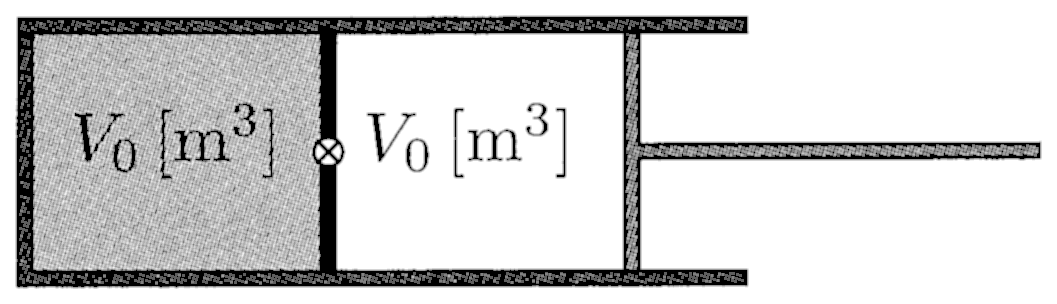
\includegraphics[keepaspectratio,width=62mm]{fig/ch17_a29_1.png}
       \end{center}
       よって，左側の空間と右側の空間を一つの系だとみなすと，この系は外界との仕事のやり取り，熱のやり取りがない．内部エネルギーの変化量を$\Delta U\U{J}$とすると，熱力学第一法則より$\Delta U=0+0$となる．内部エネルギーは絶対温度に比例するので，全体に拡がる前後で温度変化はなく，変化後の気体の温度を$T_1\U{K}$とおくと，
       \[T_1=T_0\U{K}\Ans\]
       また，このときの気体の圧力を$p_1\U{Pa}$とする．最終的には容器全体に気体が一様に拡がっているので，全体に対して状態方程式を立てることができ，
       \[p_1\cdot 2V_0=nRT_0\]
       \begin{center}
       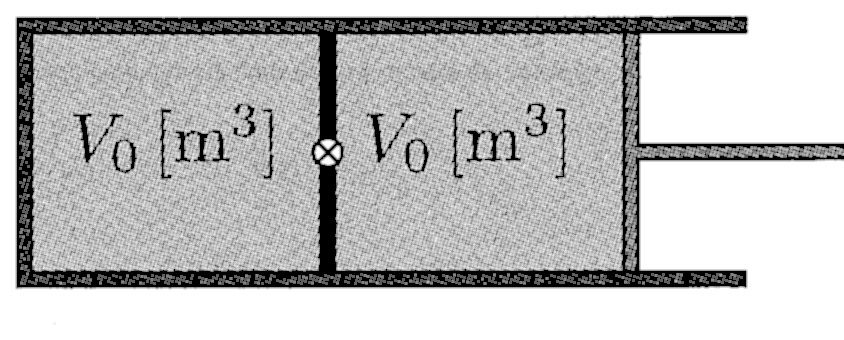
\includegraphics[keepaspectratio,width=54mm]{fig/ch17_a29_2.png}
       \end{center}
       これと最初の状態方程式とを組み合わせて解くと，
       \[p_1=\frac{1}{2}p_0\U{Pa}\Ans\]
\ko{2} バルブを全開にしてから取っ手をゆっくりと引く場合，バルブを通して気体は右側へと十分に拡散することができるので，例えば右側の体積が$V\U{m^3}$となったときには，気体は次の図のように左側と右側とにムラなく広がっている．
       \begin{center}
       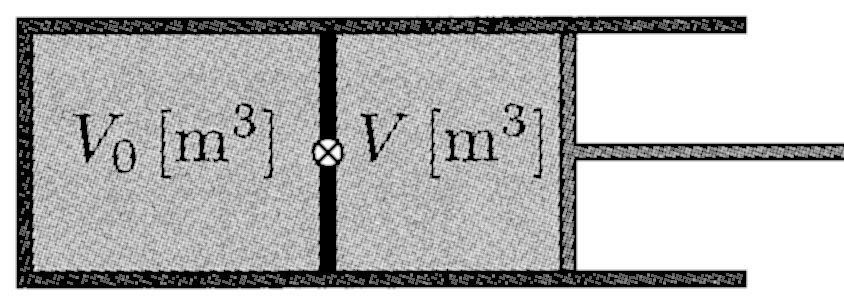
\includegraphics[keepaspectratio,width=54mm]{fig/ch17_a29_3.png}
       \end{center}
       すなわち，この状態変化ではバルブは存在しないのと全く同様にみなせるので，この状態変化は次図と全く同じものとみなせる．
       \begin{center}
       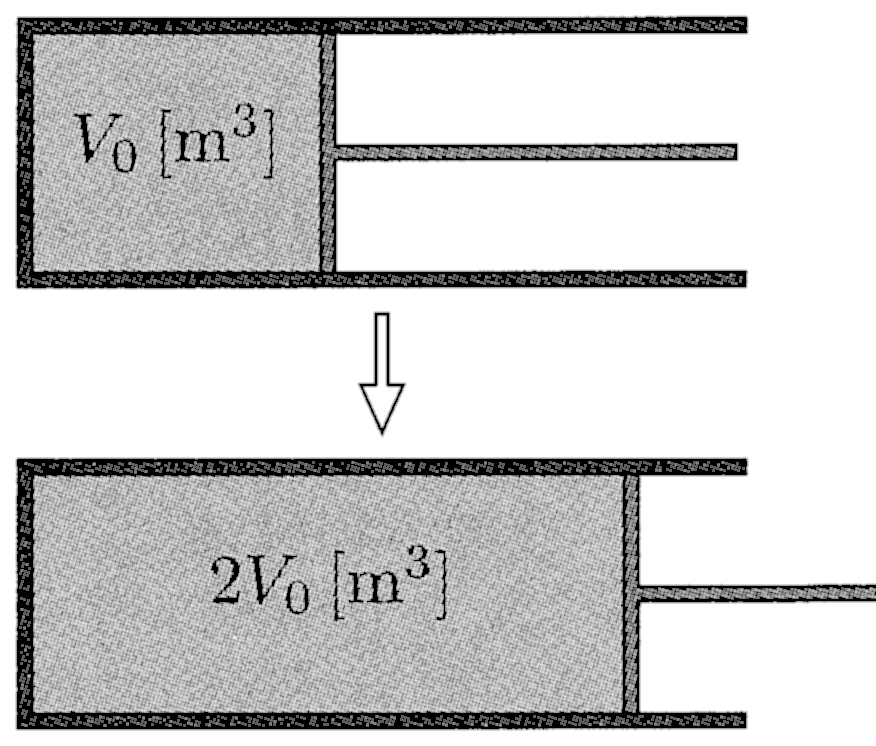
\includegraphics[keepaspectratio,width=52mm]{fig/ch17_a29_4.png}
       \end{center}
       よって，この断熱変化に対してはポアソンの式を適用することができる．この気体の比熱比$\gamma$は
       \[\gamma=\frac{C_P}{C_V}=\frac{C_V+R}{C_V}=1+\frac{R}{C_V}\]
       で与えられるので，終状態の圧力を$p_2\U{Pa}$とすると，ポアソンの式より，
       \[p_0V_0^\gamma=p_2(2V_0)^\gamma\]
       が成立する．これを解いて，
       \[p_2=\frac{1}{2^\gamma}p_0=\frac{1}{2^{1+R/C_V}}p_0\U{Pa}\Ans\]
       また，終状態での温度を$T_2\U{K}$とおくと，状態方程式を立てると，
       \[p_2\cdot 2V_0=nRT_2\]
       よって，
       \[T_2=\frac{1}{2^{R/C_V}}T_0\U{K}\Ans\]
       \begin{bsHosoku}{参考}
       二つの変化それぞれの正しい解法は上述した通りだが，ではなぜ(1)の場合にポアソンの式が利用できないのか？

       それは，(1)の状態変化では，変化途中（すなわち左から右へと気体が拡散している途中）において，気体全体を一つの均一系とみなすことができないからである．

       次の図にあるように，気体が左から右へ拡散していく途中では左の気体の方が気体の密度，圧力が高い．そのため，左，右のそれぞれについて状態方程式を立てることはできるが，左＋右をひとくくりにして状態方程式を立てることができない（圧力が共通ではないから）．
       \begin{center}
       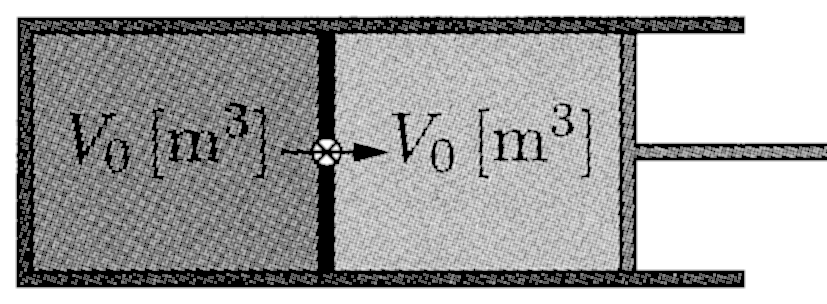
\includegraphics[keepaspectratio,width=54mm]{fig/ch17_a29_ref.png}
       \end{center}
       ポアソンの式の導出では気体全体に対しての状態方程式を利用しているので，(1)のような断熱自由膨張に対してはポアソンの式を利用することができないのである．
       \end{bsHosoku}
\end{komon}

\Rank{C問題}
\MonN{30}{気体の一般的な状態変化}\par\nopagebreak
\begin{sisin}
本問はバネがあるため，気体の状態変化は定積，定圧，定温，断熱のいずれにも当てはまらない．このような場合には，全ての状態変化に対して成立する次の基本的な流れに従って考えよ．
\begin{list}{}{\setlength{\leftmargin}{1.6zw}\setlength{\itemsep}{0.3mm}\setlength{\topsep}{0.6mm}\setlength{\parsep}{0pt}}
\item[\MARU{1}] $w=\displaystyle\int_{V_{\mathrm{start}}}^{V_{\mathrm{end}}}P(V)dV$の計算
\item[\MARU{2}] $\Delta U=nC_V\Delta T$の計算
\item[\MARU{3}] 熱力学第一法則$\Delta U=Q+(-w)$の立式
\end{list}
\end{sisin}
\KaiHead
問題の図にある，バネが距離$x\U{m}$だけ縮んだ途中状態における気体の圧力を$P(x)$とすると，ピストンに対して作用する力のつり合いより，
\[P(x)S=P_0S+kx\]
これより，
\[P(x)=P_0+\frac{kx}{S}\U{Pa}\]
また，このときの体積は
\[V(x)=S(l_0+x)\U{m^3}\]
封入されている気体のモル数を$n\U{mol}$とすると，最初の状態の状態方程式は
\[P_0\cdot Sl_0=nRT_0\]
である．
\begin{komon}
\ko{1} 終状態，すなわち$x=a\U{m}$のときは，
       \[P_1=P(a)=P_0+\frac{ka}{S}\U{Pa}\Ans\]
       であり，このときの気体の状態方程式は
       \[P_1\cdot S(l_0+a)=nRT_1\]
       これと最初の状態の状態方程式を組み合わせて解くと，
       \[T_1=\left(1+\frac{ka}{P_0S}\right)\left(1+\frac{a}{l_0}\right)T_0\U{K}\Ans\]
\ko{2} この状態変化で気体がする仕事は，積分を用いて
       \[w=\int_{Sl_0}^{S(l_0+a)}P(V)dV\]
       で求められる．この式の積分変数を$V$から$x$に変えると，
       \[\frac{dV}{dx}=S\;\Leftrightarrow\;dV=Sdx\]
       \[V=S(l_0+a)\;\Leftrightarrow\;x=a\]
       \[V=Sl_0\;\Leftrightarrow\;x=0\]
       であるから，
       \[\begin{aligned}
         w&=\int_0^a\left(P_0+\frac{kx}{S}\right)Sdx\\
          &=\int_0^a(P_0S+kx)dx\\
          &=P_0Sa+\frac{1}{2}ka^2\U{J}\Ans
       \end{aligned}\]
       \begin{chuu}
       圧力$P$を体積$V$で表してもよい．
       \[P(x)=P_0+\frac{kx}{S}\U{Pa}\]
       \[V(x)=S(l_0+x)\U{m^3}\]
       の2式から$x$を消すと，
       \[P(V)=P_0+\frac{k}{S}\left(\frac{V}{S}-l_0\right)\U{Pa}\]
       が得られる．これをもとに$p-V$図を描き，その面積から仕事を求めることができる．
       \end{chuu}
\ko{3} この状態変化での内部エネルギーの増加は
       \[\Delta U=nC_V(T_1-T_0)\]
       であり，熱力学第一法則$\Delta U=Q+(-w)$を利用すると，
       \[\begin{aligned}
         Q&=nC_VT_0\left(\frac{ka}{P_0S}+\frac{a}{l_0}+\frac{ka^2}{P_0Sl_0}\right)\\
          &\qquad\qquad\qquad+P_0Sa+\frac{1}{2}ka^2\U{J}\\
          &=\frac{C_V}{R}kal_0+\frac{2C_V+R}{2R}ka^2\\
          &\qquad\qquad\qquad+\frac{C_V+R}{R}P_0Sa\U{J}\Ans
       \end{aligned}\]
\end{komon}

\end{multicols}
